%openany: no empty pages between chapters/parts
%oneside: for ebook reading, change to towside for printing !!!!!!!!!!!!!! <-----------
\documentclass[openany, oneside, a4paper]{memoir}


%font specific includes
%\setromanfont{FreeSerif}
%\setsansfont{FreeSans}
%\setmonofont{FreeMono}
%greek support with word "brakes"
\usepackage{fontspec}
\usepackage{xunicode}
\usepackage{xgreek}
\setmainfont[Mapping=TeX-text]{Times New Roman}




%absract specific declarations (abstract is usde in the frontmatter
\usepackage{abstract}
\renewcommand{\abstractname}{}  % clear the title
%\renewcommand{\absnamepos}{empty} % originally center

%empty chapter names
\renewcommand{\chaptername}{}

%specifying table of contents
% \renewcommand{\contentsname}{Περιεχόμενα}
% \renewcommand*{\cftchapterleader}{\hfill}
%specifying max depth table of containts should contain
% \maxtocdepth{subsubsection} %dotted style in subsections too
\setsecnumdepth{subsection}
\setcounter{secnumdepth}{3}
\setcounter{tocdepth}{3}

%used in includegraphics command
\usepackage{graphicx}
\newcommand{\HRule}{\rule{\linewidth}{2.5mm}}



%%%%%%%%%%%%%%%%%%%%%%%%%%%%%%%%%%%%%%%%%% DOCUMENT BEGINS HERE %%%%%%%%%%%%%%%%%%%%%%%%%%%%%%%%%%%%%%%%%%%%%%%%%%%%%%%
\begin{document}
\frontmatter
%titlepage + prologue + abstract

%%%%%%%%%%%%%%%%%%%%%%%%%%%%%%%%%%%%%%%%%%%%%%% titlepage %%%%%%%%%%%%%%%%%%%%%%%%%%%%%%%%%%%%%%%%%%%%%%%%%%%%%%%
\begin{titlingpage}
\begin{center}

% Upper part of the page

\includegraphics[width=0.25\textwidth]{images/upatras_logo.jpg}\\[1cm]

\HUGE 	ΠΑΝΕΠΙΣΤΗΜΙΟ ΠΑΤΡΩΝ\\
\LARGE	Πολυτεχνική Σχολή\\
\Huge	Τμήμα Μηχανικών Ηλεκτρονικών Υπολογιστών και Πληροφορικής\\[1.5cm]

\LARGE Προπτυχιακή Διπλωματική Εργασία\\[0.1cm]


% Title
\HRule \\[0.4cm]
{ \HUGE \bfseries Αποδοτική Διαχείρηση Ενέργειας σε Ασύρματα Επαναφορτιζόμενα Δίκτυα Αισθητήρων}\\[0.4cm]

\HRule \\[0.5cm]

% Author and supervisor
\begin{minipage}{0.4\textwidth}
\begin{flushleft} \large
\emph{Συγγραφέας:}\\
Φίλιππος Βασιλάκης, \\AM: 3895\\ vasilakis@ceid.upatras.gr
\end{flushleft}
\end{minipage}
\begin{minipage}{0.4\textwidth}
\begin{flushright} \large
\emph{Επιβλέπων:} \\
Σωτήρης Νικολετσέας, \\Επίκουρος Καθηγητής\\ nikole@cti.gr
\end{flushright}
\end{minipage}

\vfill

% Bottom of the page
{\large Μάιος 2012}

\end{center}

\end{titlingpage}
%%%%%%%%%%%%%%%%%%%%%%%%%%%%%%%%%%%%%%%%%%%%%%% titlepage ended %%%%%%%%%%%%%%%%%%%%%%%%%%%%%%%%%%%%%%%%%%%%%%%%%%%%%%%
\begin{comment}
% \frontmatter
\chapter{Πρόλογος}
Ένα Ασύρματο Δίκτυο Αισθητήρων(ΑΔΑ) αποτελείται από πολλές διασπαρμένες μικρές, αυτόνομες, ασύρματα συνδεδεμένες συσκευές. Κάθε συσκευή λαμβάνει μετρήσεις από το
άμεσο περιβάλλον της όπως θερμοκρασία, υγρασία, κλπ ενώ ταυτόχρονα οι πόροι όπως η μνήμη και η ενέργεια που έχει στη διάθεσή της η κάθε συσκευή είναι πολύ
περιορισμένοι.
Η ιδέα αναπτύχθηκε στα τέλη της δεκαετίας 1990 και τα πρώτα πειραματικά δίκτυα κατασκευάστικαν στις αρχές του 2000. Σε αυτά τα χρόνια η έρευνα επικεντρώθηκε κυρίως
στην διατύπωση των θεμελιωδών ιδιοτήτων που χαρακτηρίζουν ένα Ασύρματο Δίκτυο Αισθητήτων. Από τους πρώτους ερευνητές που άρχισαν να ασχολούνται με αυτά τα
δίκτυα υπήρχε η κοινή διαπίστωση οτι οι διαφορές από τα κλασσικά Ασύρματα Δίκτυα(ad-hoc networks) ήταν πολύ μεγάλες κυρίως στους στόχους του κάθε δικτύου.
Διατυπώθηκαν τα πρώτα προβλήματα που έπρεπε να λυθούν σε ένα τέτοιο δίκτυο τα οποία κυρίως αφορούσαν την εξοικονόμηση ενέργειας.

Σχεδόν μία δεκαετία μετά, τα Ασύρματα Δίκτυα Αισθητήρων ακόμα προκαλούν τους επιστήμονες στο θέμα της ελαχιστοποίησης της κατανάλωσης της ενέργειας. Αποδοτικοί
αλγόριθμοι, καινοτόμες τοπολογίες, ριζοσπαστικές ιδέες που ξεφεύγουν από τα κλασσικά μοντέλα, όπως κίνηση κάποιων αισθητήρων, τελευταίως και η εκμετάλευση
εναλλακτικών μορφών ενέργειας έχουν χρησιμοποιηθεί προκειμένου να μειώσουν την κατανάλωση ενέργειας στο δίκτυο. Το ανολοκλήρωτο όνειρο της επιστημονικής κοινότητας
είναι να γίνει πραγματικότητα ένα ΑΔΑ στο οποίο όλες οι συσκευές να έχουν μικρή παρόμοια κατανάλωση ενέργειας και χρόνο ζωής το άπειρο.

Τελευταία, μία καινούργια ανακάλυψη έρχεται να αναταράξει τα ΑΔΑ: Η Ασύρματη μεταφορά ενέργειας.

\chapter{Ευχαριστίες}
\begin{abstract}
Θα ήθελα να ευχαριστήσω τον κ. Σωτήρη Νικολετσέα, Επίκουρο Καθηγητή του Πανεπιστημίου Πατρών, για την επίβλεψη της παρούσας εργασίας, τη καθοδήγηση και την
εμπιστοσύνη που επέδειξε στο πρόσωπό μου όταν του ζήτησα μία καινοτόμα διπλωματική. Η εμπίστοσύνη αυτή σίγουρα με έκανε να δουλέψω ακόμα σκληρότερα. Θα ήθελα
να ευχαριστήσω τον Διδακτορικό Μάριο Αγγελακόπουλο ο οποίος με την πολυετή εμπειρία και τις σοφές παρατηρήσεις του συνέβαλε σημαντικά στα παρακάτω αποτελέσματα.
Επίσης ευχαριστώ τον συνάδελφο, απόφοιτο, Φάνη Ράπτη που βοήθησε σημαντικά να βγουν έγκαιρα τα αποτελέσματα. Είμαι σίγουρος οτι έχει λαμπρό μέλλον ως μέλος
της υπόλοιπης ομάδας.

Πάνω από όλους όμως θα ήθελα να ευχαριστήσω τους γονείς μου για τις συμβουλές τους και την στήριξη και που μου παρείχαν καθόλη την
διάρκεια των σπουδών μου. Χωρίς αυτούς τίποτα από όλα αυτά δεν θα είχε πραγματοποιηθεί.

\end{abstract}
\newpage
\end{comment}
\tableofcontents
% \mainmatter

\mainmatter
%1st chapter



\chapter{Εισαγωγή στα Ασύρματα Δίκτυα Αισθητήρων}

\section{Εισαγωγή}
Στα τέλη της δεκαετίας του 1990 αναπτύχθηκαν στον κόσμο των υπολογιστών και της πληροφορικής, αμφότερα τα όραματα "Περιρρέουσα Νοημοσύνη" ( Ambient Intelligence ) και
του "Διάχυτου Υπολογισμού" (Pervasive Computing ή πιο συχνά Ubiquitus Computing).
Η έννοιες αυτές αναφέρονται αφηρημένα σε ένα περιβάλλον το οποίο είναι ικανό να "νιώθει" και να καταλαβαίνει τους ανθρώπους, και γενικότετερα
τις οντότητες, που βρίσκονται σε αυτό \cite{ambient}.
Λίγο πιο συγκεκριμένα, σε ένα τέτοιο περιβάλλον υπάρχουν αυθαίρετα πολλές συσκευές οι οποίες επικοινωνούν και συνεργάζονται μεταξύ τους με κοινό στόχο την εξυπηρέτηση
του ανθρώπου.
Η εξυπηρέτηση αυτή έχει να κάνει από τις καθημερινές εργασίες, όπως αυτόματος οπλισμος/αφοπλισμός συναγερμού, αυτόματο πότισμα, αυτόματο άνοιγμα των φώτων, παράθυρων
και ρύθμιση της θερμοκρασίας του σπιτιού όταν εισέρχεται ο ιδιοκτήτης του, αλλά και πιο προηγμένες τεχνολογιές όπως αντιμετώπιση μιας πυρκαγιάς σε ένα δημόσιο κτήριο
ή υπόδειξη νέων κατάλληλων
προιόντων σύμφωνα με τις καταναλωτικές συνήθειες μιας οικογένειας.

Γίνεται επομένως εμφανές οτι το όραμα αυτό, αν και αρκετά ελπιδοφόρο, στην τελική του μορφή περιλαμβάνει πολλές τεχνολογίες και επιστήμες μαζί, αποτελεί δηλαδή ένα
σχετικά καινούργιο διεπιστημονικό πεδίο.
Συγκεκριμένα για την υλοποίηση του οράματος χρειάζονται βασικά εργαλεία (γνώσεις και αλγόριθμοι) από επιστήμες όπως η Θεωρία Πληροφορίας, της Ανοχής σε Σφάλματα,
τα Δίκτυα, τα Ασύρματα Κινητά Δίκτυα, τα Ασύρματα Δίκτυα Αισθητήρων, τα Κατανεμημένα Συστήματα, της Ασφάλειας και πολλών άλλων. Ένας παραστατικός συνδυασμός αυτών
των επιστημών με τελικό αποτέλεσμα αυτών τον Διάχυτο Υπολογισμό φαίνεται στην εικόνα \ref{fig:pervasive}.

\begin{figure}[h]
	\centering
	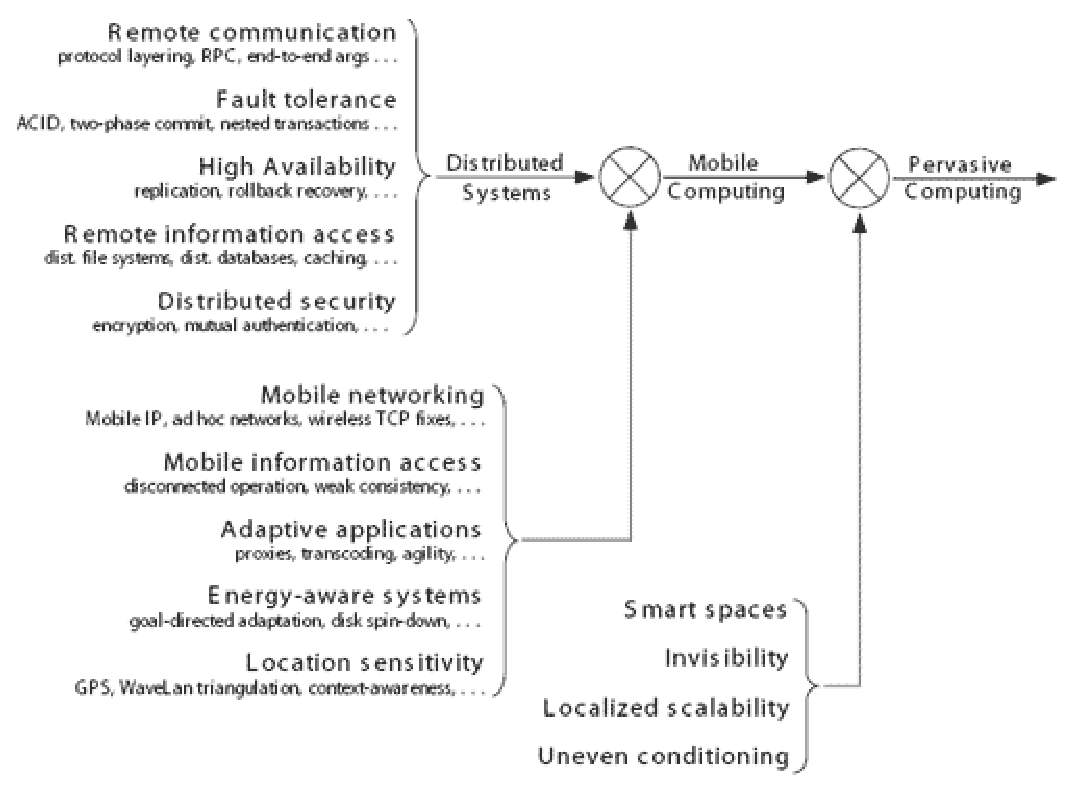
\includegraphics[width=0.8\textwidth]{images/pervasive_computing.eps}
  \caption[Caption for LOF]{Ο Διάχυτος Υπολογισμός ως συνδυασμός επιστημών\footnotemark}
	\label{fig:pervasive}
\end{figure}

Ένα από τα πιο σημαντικά, αν όχι το πιο σημαντικό, εργαλεία του Διάχυτου Υπολογισμού είναι τα Ασύρματα Δίκτυα Αισθητήρων(ΑΔΑ).
Τα ΑΔΑ αποτελούνται από έναν μεγάλο αριθμό κόμβων οι οποίοι καλύπτουν επαρκώς το περιβάλλον το οποίο είναι σε επιτήρηση.
Είναι το υποσύστημα το οποίο καταγράφει όλες τις πληροφορίες από το περιβάλλον αλλά και ταυτόχρονα είναι το ίδιο υποσύστημα που εκτελεί τις λειτουργίες που είναι
απαραίτητες κάθε στιγμή.
Ένα από τα κρισιμότερα συστατικά των ΑΔΑ είναι ο αισθητήρας: είναι το υποσύστημα του κόμβου το οποίο μετατρέπει μια φυσική ποσότητα όπως η υγρασία, η θερμοκρασία
κλπ σε ηλεκτρονικό δεδομένο.
Η επιστημονική κοινότητα από τις αρχές του 2000, αφού έχει μελετήσει σε βάθος τις προηγούμενες επιστήμες, σε σχέση με τα ΑΔΑ, όπως τα Δίκτυα, Ασύρματα Δίκτυα,
Κατανεμημένα Συστήματα κλπ έχει εστιάσει μεγάλο μέρος της προσοχή της στα Ασύρματα Δίκτυα Αισθητήρων αφού αποτελούν απαραίτητο εργαλείο για τον Διάχυτο Υπολογισμό.

\footnotetext{Η εικόνα παρουσιάζεται στην ιστοσελίδα του εργαστηρίου Διάχυτου Υπολογισμού του πανεπιστημίου Carnegie Mellon (CMU)}

Τα τελευταία αυτά 10 χρόνια, τα Ασύρματα Δίκτυα Αισθητήρων γνώρισαν τρομερή πρόοδο σε όλο το διάστημα. Εφευρέθηκαν μαθηματικά μοντέλα που προσομοιώνουν πλήρως τα
ΑΔΑ\cite{geometric_graphs}, αλγόριθμοι οι οποίοι εκμεταλεύονται πλήρως τις ιδιότητές τους ώστε να έχουν καλύτερη απόδοση, άνω και κάτω φράγματα σε αποδόσεις
αλγορίθμων και πολλά άλλα.
Ο πιο σημαντικός περιορισμός τους, ο οποίος διαπιστώθηκε από την αρχή της έρευνας, είναι οι περιορισμένοι πόροι των κόμβων ειδικά σε θέματα ενέργειας.
Η περιορισμένη χωρητικότητα ενέργειας ενός κόμβου είναι το σημείο κλειδί το οποίο μάλιστα διαφοροποιεί τα ΑΔΑ από τα κλασσικά Ασύρματα Δίκτυα.
Επομένως η περισσότερη έρευνα πανω στα ΑΔΑ, ακόμα και 10 χρονια μετά, έχει σχέση με την ελαχιστοποίηση της κατανάλωσης της ενέργειας. Είναι πλέον αποδεκτό οτι με την
σημερινή τεχνολογία τα ΑΔΑ δεν γίνεται να λειτουργούν επ'άπειρον χωρίς την ανθρώπινη παρέμβαση κάτι που επηρεάζει σημαντικά το όραμα του Διάχυτου Υπολογισμού.
Διότι αν ο κάθε κόμβος σε ένα ΑΔΑ χρειάζεται ανθρώπινη παρέμβαση ανά τακτά χρονικά διαστήματα τότε το κόστος του συνολικού συστήματος αυξάνεται σημαντικά, ένας τομέας
που από την έναρξη μαζικής παραγώγής τέτοιων συστημάτων λαμβάνεται σοβαρά υπόψη και καθορίζει τελικά την επιτυχία τους. Όμως ακόμα και αν εξαιρέσουμε τον παράγοντα
του κόστους, ένα ΑΔΑ στο οποίο οι κόμβοι λόγω περιορισμένης ενέργειας διακόπτουν τη λειτουργία τους απρόσμενα μετά το ίδιο το δίκτυο γίνεται αναξιόπιστο
αποτυγχάνοντας τον αρχικό του στόχο: να βοηθά τον άνθρωπο.

Ωστόσο μια καινούργια τεχολογία που εφευρέθηκε από τους επιστήμονες του MIT \cite{power_mit_1} έρχεται να αλλάξει άρδην τις προσδοκίες στο πεδίο των ΑΔΑ. Η τεχνολογία
αυτή επιτρέπει την ασύρματη μετάδοση ενέργειας από μια πηγή σε έναν δέκτη με πολύ μικρές απώλειες ενέργειας. 






\section{Ασύρματα Δίκτυα Αισθητήρων(ΑΔΑ)}
Ένα Ασύρματο Δίκτυο Αισθητήρων(ΑΔΑ) αποτελείται από αυτόνομους κατανεμημένους κόμβους(ή αισθητήρες) όπου ο καθένας λαμβάνει μετρήσεις για το κοντινότου περιβάλλον,
όπως θερμοκρασία, υγρασία, επίπεδα θορύβου, σεισμικές δονήσεις, πίεση ακόμα και κίνηση με την προϋπόθεση πάντα οτι υπάρχει το απαραίτητο υλικό πάνω στον κόμβο ωστε
να μπορεί να λάμβάνει εκάστοτε μέτρηση.
Οι κόμβοι λαμβάνουν μετρήσεις περιοδικά με περίοδο που εξαρτάται από το είδος το δικτύου και ρυθμίζεται από τον αρχικό σχεδιαστή του δικτύου.
Για ένα δίκτυο οι κόμβοι μπορεί να λαμβάνουν μετρήσεις ανά μια ώρα ενώ σε κάποιο άλλο δίκτυο οι αισθητήρες μπορεί να λαμβάνουν μετρήσεις ανα ένα δευτερόλεπτο.
Σε ένα ΑΔΑ σχεδόν πάντα θεωρείται οτι υπάρχει ένα ακόμα πολύ σημαντικό στοιχείο: η Πηγή.
Ο κάθε κόμβος αφού λάβει και καταγράψει ένα μέγεθος μετρήσεων στέλνει τα δεδομένα αυτά, δομημένα σε πακέτα μέσα από ένα πρωτόκολλο δρομολόγησης, στην Πηγή
χρησιμοποιώντας ως διαμελοσαβητές άλλους κόμβους.
Θα πρέπει να αναφερθεί οτι ο κάθε κόμβος δεν γνωρίζει την συνολική διαδρομή που θα ακολουθήσουν τα πακέτα αλλά γνωρίζει μόνο τον πρώτο γείτονα στον οποίο στέλνει κάθε
φορά ένα πακέτο που έχει προορισμό την Πηγή. Ένα παράδειγμα ενός ασύρματου δικτύου αισθητήρων φαίνεται στην εικόνα \ref{fig:farm}.

\begin{figure}[h]
	\centering
	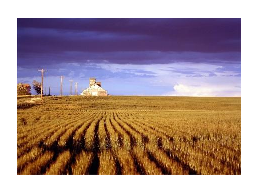
\includegraphics[width=0.8\textwidth]{images/farm.eps}
	\caption{Ένα τυπικό σενάριο ενός ΑΔΑ}
	\label{fig:farm}
\end{figure}

Τα βασικά κριτήρια που χαρακτηρίζουν ένα δίκτυο ως ΑΔΑ είναι τα εξής:
\begin{itemize}
\item μεγάλοι περιορισμοί ως προς την κατανάλωση ενέργειας για τους κόμβους
\item ικανότητα του δικτύου να μπορεί να αντιμετωπίζει αποδοτικά δυσλειτουργίες και σφάλματα κόμβων
\item ικανότητα αντιμετώπισης αποτυχιών και προβλήματα επικοινωνίας μεταξύ κόμβων
\item ανομοιογένεια ως προς τους κόμβους
\item τοπικότητα στην πληροφορία
\item επεκτασιμότητα του δικτύου σε πολύ μεγάλα μεγέθη
\item εύκολη εγκατάσταση και χρήση του συνολικού δικτύου από έναν χειριστή
\end{itemize}
Ο αριθμός των κόμβων μπορεί να κυμαίνεται από μερικές εκατοντάδες μέχρι και αρκετές χιλιάδες.
Η κατανομή των κόμβων, δηλαδή ο τρόπος που τοποθετούνται, συνήθως είναι ομοιόμορφη αλλά αυτό δεν ισχύει πάντα. Για παράδειγμα έχει αποδεχτεί οτι μια διαφορετική
κατανομή όπως η Gaussian μπορεί να έχει καλύτερη απόδοση σε ένα ΑΔΑ, όσον αφορά κάποια συγκεκριμένα χαρακτηριστικά \cite{gaussian_sensors}.
Ο κάθε κόμβος αποτελείται συνήθως από κάποια τυπικά μέρη:
\begin{itemize}
\item πομπό/δέκτη που να χρησιμοποιεί χαμηλής ενέργειας ασύρματα πρωτόκολλα
\item μικροελεγκτή χαμηλής κατανάλωσης ενέργειας, από πολύ απλούς των 8bit μέχρι και σύχρονους με μεγάλη υπολογιστική δύναμη. Το κύριο χαρακτηριστικό τους είναι η
μικρή κατανάλωση ενέργειας
\item μπαταρία και γενικά ένας πόρος ενέργειας
\item αισθητήρες όπως θερμόμετρο, βαρόμετρο, κάμερα κλπ
\end{itemize}
Αν και υπάρχει η τεχνολογία να φτιαχτεί το υλικό ενός κόμβου σε μέγεθος "ψείρας", οι μπαταρίες αυξάνουν δραματικά το μέγεθος ούτως ώστε ένας κόμβος να λειτουργεί
απροβλημάτιστα για πλύ καιρό.
Επίσης θα πρέπει να σημειωθεί οτι, αν και θεωρούμε οτι υπάρχουν κάποιοι περιορισμένοι πόροι όσον αφορά το υλικό όπως για παράδειγμα τις δυνατότητες
του μικροεπεξεργαστή και κατα συνέπεια του μικροελεγκτή που φέρει ένας κόμβος, στα ΑΔΑ δεν μελετώνται περιπτώσεις όπου οι κόμβοι δεν έχουν έλεγχο της κίνησής τους ή
δεν έχουν καθόλου μνήμη και ικανότητα εκτέλεσης βασικών πράξεων.
Τέτοιες περιπτώσεις υπάγονται σε άλλα μοντέλα όπως τα πρωτόκολλα πληθυσμών \cite{population_protocols}.

Η Πηγή είναι ένα ξεχωριστό στοιχείο του δικτύου, το οποίο έχει τεράστια υπολογιστική ικανότητα σε σχέση με τους κόμβους, δεν έχει κανέναν περιορισμό πόρων ενώ
ταυτόχρονα έχει εμβέλεια επικοινωνίας
πολύ μεγαλύτερη από τους κόμβους.
Σε μερικά δίκτυα η Πηγή συμμετέχει στο πρωτόκολλο δρομολόγησης ή βοηθάει μερικώς το συνολικό δίκτυο χρησιμοποιώντας τα ιδιαίτερα χαρακτηριστικά της.
Στην Πηγή φθάνουν τελικά όλες οι πληροφορίες και είναι υπεύθυνη για την διαχείρηση αυτών των πληροφοριών όπως για παράδειγμα εκτέλεση ειδικών
ερωτημάτων(queries) επάνω στα δεδομένα για ασφαλή και γρήγορη εξαγωγή συμπερασμάτων για το δίκτυο.

Τα βασικά Ασύρματα Δίκτυα Αισθητήρων σταματάνε σε αυτό το σημείο.
Ο διαχειρισμός των δεδομένων καθώς και η εξαγωγή μετα-πληροφοριών από αυτά τα δεδομένα κλπ αποτελούν μέρη των διεπιστημονικών πεδίων του Διάχυτου Υπολογισμού και
Περιρρέουσας Νουμοσύνης.
Γίνεται επομένως σαφές λόγω του οτι τα ΑΔΑ αποτελούν το πιο κρίσιμο συστατικό για τις προαναφερθήσες επιστήμες.

Τέλος να σημειωθεί οτι γενικώς στα ΑΔΑ θεωρείται οτι οι αισθητήρες έχουν συνεργατικές τάσεις, δηλαδή συνολικά το δίκτυο έχει κοινό στόχο.
Αντίθετα πολύ σπάνια μελετώνται περιπτώσεις όπου ο κάθε κόμβος κοιτάει μεμωνομένα και εγωιστικά το δικό του συμφέρον.
Η ανάλυση αυτών των περιπτώσεων χρησιμοποιεί συνήθως θεωρία παιγνίων \cite{game_theroy_sensor}, ενώ υποδεικνύει ένα πλήρως ανομοιογενές δίκτυο διαφορετικό από την
αρχική φιλοσοφία των ΑΔΑ.

\section{Το Κίνητρο και Σύντομη Ιστορία των ΑΔΑ} \label{sec:history}
Το βασικό κίνητρο των ΑΔΑ ήταν κατα κύριο λόγο οι στρατιωτικές εφαρμογές.
Επισκόπηση του πεδίου μάχης, αναγνώριση στόχων, παρακολούθηση και καταγραφή των στρατιωτικών δυνάμεων και των διαθέσιμων πυρομαχικών τους ήταν από τις πρώτες
εφαρμογές που είχαν πυροδοτήση την απόσπαση κονδυλιών, από κυβερνήσεις δυνατών κρατών, για την έρευνα τέτοιων μηχανισμών.
Συγκεκριμένα η πρώτη πραγματική εύρευνα πάνω στα δίκτυα αισθητήρων ξεκίνησε μέσα στην δεκαετία του 1980 στην υπηρεσία του υπουργίου Αμύνης των Η.Π.Α, την DARPA
(Defense Advanced Research Projects Agency).
Η υπηρεσία αυτή ξεκίνησε ένα καινούργιο πρόγραμμα το οποίο λεγόταν Κατανεμημένα Δίκτυα Αισθητήρων (DSN, Distributed Sensor Networks).
Ταυτόχρονα το ARPANET (Advanced Research Projects Agency Network) δίκτυο ήταν πλήρως λειτουργικό με 200 πανεπιστήμια και ερευνιτικά κέντρα συνδεδεμένα.
Η βασική ιδέα των DSN ήταν ένα δίκτυο πολλών κατανεμημένων συνδεδεμένων κόμβοι οι οποίοι συνεργάζονταν μεταξύ τους αλλά ο κάθε κόμβος λειτουργούσε ανεξάρτητος.
Το πρωτόκολλο δρομολόγησης που χρησιμοποιήθηκε βασιζόταν στην μέθοδο της πλημύρας.

Αν συνυπολογισθεί οτι εκείνη την περίοδο δεν υπήρχαν προσωπικοί υπολογιστές, πόσο μάλλον φορητοί υπολογιστές, ενώ το Ethernet μόλις άρχιζε και αποκτούσε φήμη, το
πρόγραμμα DSN ήταν πολύ φιλόδοξο.
Η τεχνολογία για την υλοποίση αυτού του εγχειρήματος είχε βρεθεί σε ένα σχετικά πρόσφατο συνέδριο\cite{1978DSN}.
Ουσιαστικά περιελάμβανε έναν αισθητήρα ήχου, ικανότητα αποστολής και λήψης σημάτων χαμηλής ενέργειας και το απαραίτητο λογισμικού κατανεμημένου χαρακτήρα.
Επιστήμονες από το πανεπιστήμιο Carnegie Mellon (CMU), εστίασαν το ενδιαφέρον τους στη κατασκευή ένός λειτουργικού συστήματος το οποίο θα απευθυνόταν σε τέτοιες
συσκευές, δηλαδή συσκευές συνδεδεμένες σε ένα δίκτυο, στις οποίες υπάρχει εύκολη και ενιαία πρόσβαση στους κατανεμημένους πόρους ενός αξιόπιστου DSN συστήματος.
Το αποτέλεσμα αυτού του συστήματος ήταν να δημιουργηθεί το λειτουργικό σύστημα Mach το οποίο για την εποχή του είχε αρκετά πρωτοπόρα στοιχεία \cite{Mach} ενώ είχε
μάλιστα και κάποια περιορισμένη εμπορική επιτυχία.

Λίγο καιρό αργότερα, επιστήμονες στο πανεπιστήμιο MIT επικεντρώθηκαν στην αναγνώριση (εχθρικών) ελικοπτέρων μέσα από επεξεργασία ακουστικών σημάτων.
Το σύστημα που χρησιμοποιήσαν ήταν μικρόφωνα κατανεμημένα διάσπαρτα σε ένα χώρο τα οποία στέλναν τις πληροφορίες τους σε έναν κεντρικό υπολογιστή.
Χρησιμοποίησαν ευρετικούς αλγόριθμους και τεχνικές ταιριάσματος για να μπορέσουν να πετύχουν αποδεχτά αποτελέσματα στην αναγνώριση ελικοπτέρων.
Επιπλέον επέκτειναν το σύστημα DSN προσθέτοντας αλγόριθμούς για επεξεργασία σημάτων και τεχνικών ταιριάσματος\cite{4789229}.
Για την επίδειξη του συστήματος το εργαστήριο Lincoln στο MIT κατασκεύασε ένα πραγματικό δοκιμαστικό σενάριο για την ακουστική αναγνώριση ελικοπτέρων χαμηλής πτήσης
και αεροπλάνων \cite{aircraft}.
Χρησιμοποιήθηκαν κόμβοι που στην πραγματικότητα ήταν μικρόφωνα τα οποία έστελναν με ασύρματη τεχνολογία τα σήματα ήχου σε 3 σταθερούς υπολογιστές(επεξεργαστής
MC68000, 256KB μήμη και 512ΚΒ κοιμή μνήμη).
Στην εικόνα \ref{fig:lincoln_lab}\cite{lincoln_report} φαίνεται το δοκιμαστικό σενάριο.
Τελικά το συνολικό σύστημα δούλεψε επιτυχώςκαι κατάφερε να εντοπίσει τα χαμηλής πτήσης ελικόπτερα και αεροσκάφη.
\begin{figure}[h]
	\centering
	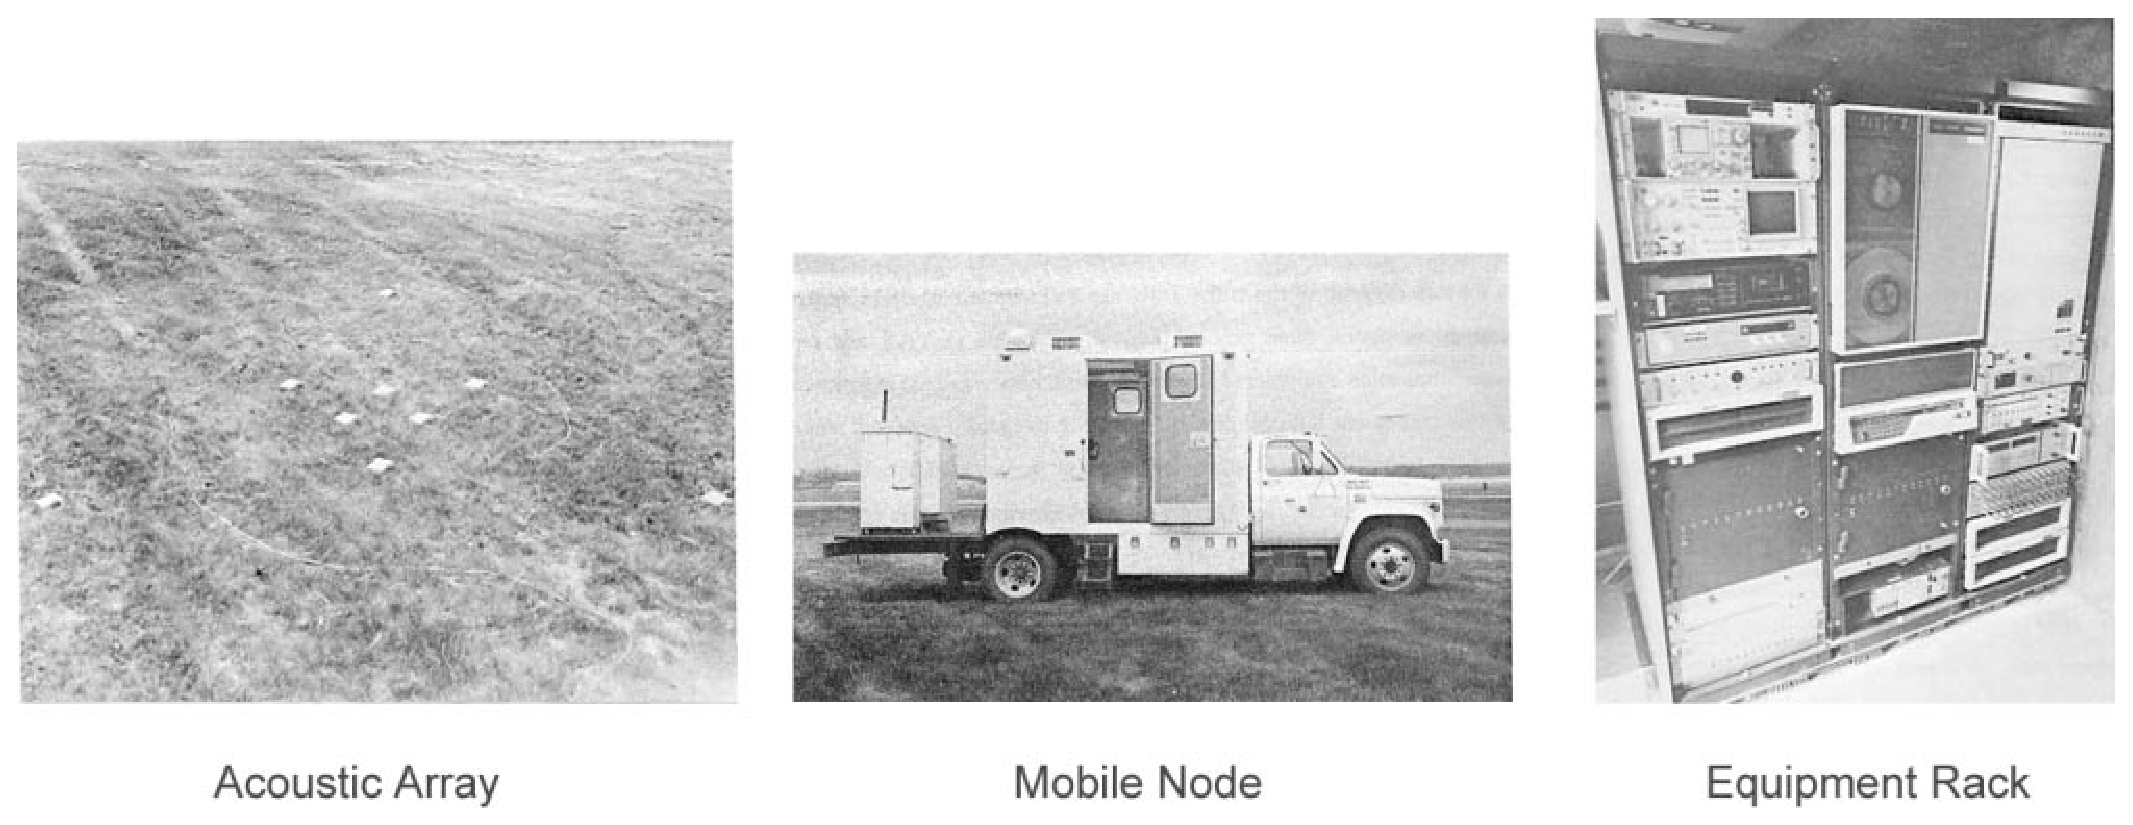
\includegraphics[width=0.8\textwidth]{images/lincoln_lab.eps}
	\caption{Tο δοκιμαστικό πείραμα του εργαστηρίου Lincoln του MIT}
	\label{fig:lincoln_lab}
\end{figure}

Ενώ οι ερευνητές είχαν κατανοήσει οτι τέτοια συστήματα θα έπρεπε να περιλαμβάνουν πολλά μικρά δίκτυα αισθητήρων τα οποία θα έχουν εκατοντάδες κόμβους, η τεχνολογία
για αυτά τα συστήματα δεν ήταν πλήρως έτοιμη.
Ωστόσο στρατιωτικοί παράγοντες είχαν αναγνωρίσει την τεράστια χρησιμότητα αυτών των συστήμάτων καθώς και την υπερτερότητα των δικτυακών όπλων: χιλιάδες αισθητήρες που
συνεργάζονται και μαζεύουν πληροφορίες σε σχέση με τον εχθρό και τις αποστέλλουν στο κέντρο επιχειρήσεων, το οποίο μπορεί να είναι χιλιόμετρα μακριά από το πεδίο
μάχης.
Το προβάδισμα αυτό θα μπορούσε να λειτουργήσει μοιραία στην εξέλιξη μιας μάχης.

Το πρώτο πραγματικό σύστημα που υλοποιήθηκε με αυτόν τον σκοπό και έχει αρκετή σχέση με τα ΑΔΑ είναι το CEC (Cooperative Engagement Capability)\nocite{cec} το οποίο
κατασκευάστηκε από το ναυτικό των Η.Π.Α. στα μέσα της δεκαετίας του 1990.
Το σύστημα αποτελείται από πολλά ραντάρ τα οποία συλλέγουν πληροφορίες για στόχους αέρος όπως αεροσκάφη, ελικόπτερα πύραυλοι κλπ.
Οι μετρήσεις αυτές αποστέλνονται σε έναν κόμβο αρχηγό ( ουσιαστικά πρόκειται για μία Πηγή) ο οποίος επεξεργάζεται και φιλτράρει τις πληροφορίες.
Ο κόμβος αυτός είναι κοινός σε όλους τους άλλους κόμβους που μαζεουν πληροφορίες.
Το σημαντικό στοιχείο του σηστήματος είναι οτι όλοι οι κόμβοι έχουν πρόσβαση σε όλες τις πληροφορές δημιουργώντας ένα πραγματικά κατανεμημνο σύστημα το οποίο δίνει
την ίδια εκόνα σε όλους τους στρατιωτικούς οι οποίοι βρίσκονται σε ένα κόμβο ο καθένας. Το σύστημα αυτό ακολούθησαν και άλλα στρατηγικά συστήματα με παρόμοιους
στόχους όπως το REΒMASS (Remote Battlefield Sensor System) και το TRSS (Tactical RemoteSensor System).


Ταυτόχρονα η τεχνολογία στους υπολογιστές εξελισσόταν ραγδαία.
Είχαν κατασκευαστεί ασύρματα δίκτυα, είχε δημιουργηθεί το Internet, οι μικροεπεξεργαστές είχαν πλέον αρκετή υπολογιστική ισχύ ενώ το υπήρχε η δυνατότητα κατασκευής
μικρουπολογιστικών συστημάτων που είχαν μέγεθος όσο μια παλάμη.
Αυτές οι εξελίξεις σε συνδυασμό με τα οράματα της Περιρρέουσας Νουμοσύνης και του Διάχυτου Υπολογισμού έκαναν τους επιστήμονες να οραματιστούν μια διαφορετική πλευρά
τον δικτύων αισθητήρων: ασύρματα δίκτυα αισθητήρων τα οποία θα συλλέγαν πληροφορίες με στόχο να βοηθήσουν τον άνθρωπο.
Τα ΑΔΑ δηλαδή θα είχαν στόχο να κάνουν πιο εύκολη την ζωή του αθνρώπου από κάθε μεριά αναλαμβάνοντας αυτά κάποιες λειτουργίες σύμφωνα με τις πληροφορίες που έχουν
συλλέξει χωρίς όμως ο άνθρωπος να αλληλεπηδρά με το συνολικό σύστημα.
Έγινε όμως αμέσως αντιληπτό οτι τέτοια συστήματα θα ήταν άμεσα ευπαθή στην διαχείρηση της ενέργειας.
Διότι ενώ όλες οι υπόλοιπες τεχνολογίες είχαν εξελιχθεί ραγδαία, η πρόοδος στις τεχνολογίες της μπαταρίας είχαν πολύ μικρότερη πρόοδο ενώ ταυτόχρονα τέτοια συστήματα
θα έπρεπε να λειτουργούν σχεδόν για πάντα χωρίς την αλληλεπίδραση του ανθρώπου.
Επίσης διαπιστώθηκε οτι αλγόριθμοι για τα κλασσικά ασύρματα δίκτυα (όπως ALOHA, slotted ALOHA κλπ) δεν θα μπορούσαν να χρησιμοποιηθούν καθώς τα ασύρματα δίκτυα έχουν
στόχο την μεγιστοποίηση της απόδοση ενώ τα ΑΔΑ έχουν στόχο την μεγιστοποίηση των χρονικών διαστημάτων που οι κόμβοι, με περιορισμένους πόρους ενέγειας, αποστέλουν
πληροφορίες προς την Πηγή.

Από το 2000 και μετά η προσοχή της επιστημονικής κοινότητας επικεντρώθηκε κυρίως στην ελαχιστοποίηση της κατανάλωσης της ενέργειας στα ΑΔΑ είτε αυτό επιτυγχάνεται
μέσα από τα πρωτόκολλα δρομολόγησης είτε από τον τρόπο ανάπτυξης των αισθητήρων είτε με οποιαδίποτε άλλη τεχνική που θα μπορούσε να κάνει τα ΑΔΑ να αντισταθούν ακόμα
περισσότερη ώρα στο χρόνο.
Επίσης ξεκίνησαν να κατασκευάζονται μαζικά αισθητήρες οι οποίοι ήταν εμπορικά διαθέσιμη για πρακτικούς και ερευνητικούς σκοπός ενώ ταυτόχρονα δημιουργήθηκε το πρώτο
λειτουργικό σύστημα ειδικά για ΑΔΑ, το TinyOS.
Άμεσα οι  πρώτες πειραματικές εφαρμογές που δημιουργήθηκαν με τα ΑΔΑ οι οποίες αφορούσαν σχεδόν όλους τους τομείς της ανθρώπινης δραστηριότητας.

%\begin{comment}
\section{Ασύρματα Δίκτυα Αισθητήρων και οι Εφαρμογές τους}
Η τεχνολογία των Ασύρματων ∆ικτύων Αισθητήρων μπορεί να εφαρμοστεί σε πολλές εφαρμογές του πραγματικού κόσμου και να φέρει στην επιφάνεια κάποιες εντελώς καινούριες.
Ενα κρίσιμο και πρωτεύον συστατικό των κόμβων των ασύρματων δικτύων αισθητήρων είναι ο αισθητήρας.
Για πολλές παραμέτρους του φυσικού περιβάλλοντος υπάρχει η κατάλληλη τεχνολογία αισθητήρα που μπορεί να ενσωματωθεί σε ένα WSN.
Οι πιο ευρέως χρησιμοποιούμενοι είναι οι αισθητήρες θερμοκρασίας, υγρασίας, ήχου, πίεσης και οι χημικοί αισθητήρες.
Μια σύντομη λίστα με τις πιο βασικές εφαρμογές παρουσιάζεται παρακάτω:
\begin{itemize}
\item \textbf{Πρόληψη Καταστροφών}: Μια από τις πιο συχνά αναφερόμενες εφαρμογές των WSNs είναι στην πρόληψη καταστροφών.
Ένα τυπικό σενάριο για εφαρμογές αυτής της κατηγορίας είναι η ανίχνευση πυρκαγιών.
Οι κόμβοι αισθητήρων είναι εξοπλισμένοι με θερμόμετρα και μπορούν να υπολογίσουν τη θέση τους τρέχοντας κάποιον αλγόριθμο εντοπισμού θέσης (localization).
Τους κόμβους αυτούς μπορούμε να τους απλώσουμε σε ένα δάσος, πετώντας τους από ένα αεροπλάνο. Έτσι σχηματίζεται ένας θερμοκρασιακός χάρτης της
περιοχής και σε περίπτωση υψηλών θερμοκρασιών και χαμηλής υγρασίας που υπονοούν πυρκαγιά ενημερώνουν τους πυροσβέστες.
\item \textbf{Έλεγχος του περιβάλλοντος και της βιοποικιλότητας} Τα WSNs μπορούν να χρησιμοποιηθούν για να ελέγχουν το περιβάλλον ως προς τους χημικούς ρύπους
ή ακόμα και για το σχηματισμό μιας εικόνας ως προς τον αριθμό των διαφορετικών ειδών πανίδας και χλωρίδας μια περιοχής.
\item \textbf{Ευφυή Κτίρια} Τα μεγάλα κτίρια συχνά καταναλώνουν μεγάλα ποσά ενέργειας εξαιτίας λανθασμένης χρήσης των συσκευών Air Condtitioning (HVAC).
Μια αποδοτικότερη, πραγματικού-χρόνου και ακριβέστερη παρακολούθηση της θερμοκρασίας, της υγρασίας και άλλων παραμέτρων μπορεί να μειώσει την κατανάλωση ενέργειας.
Επίσης, μπορούν να χρησιμοποιηθούν για την παρακολούθηση των μηχανικών καταπονήσεων σε κτίρια ή γέφυρες που βρίσκονται σε σεισμικά ενεργές Σώνες, ενώ άλλου τύπου
αισθητήρες μπορούν χρησιμοποιηθούν για τον εντοπισμό εγκλωβισμένων ανθρώπων σε περιπτώσεις σεισμού.
Οι αισθητήρες μπορούν να τοποθετηθούν στα κτίρια τη στιγμή της κατασκευής τους ή αφού έχουν κατασκευαστεί.
Σε αυτές τις εφαρμογές η εξοικονόμηση ενέργειας για τους αισθητήρες είναι πολύ σημαντική απαίτηση.
\item \textbf{∆ιαχείριση Εγκαταστάσεων} Τα WSNs μπορούν να χρησιμοποιηθούν για εφαρμογές διαχείρισης μεγάλων εγκαταστάσεων, όπως θέματα ασφαλείας.
Η είσοδος των ανθρώπων στις εγκαταστάσεις μπορεί να γίνεται χωρίς κλειδιά, αλλά με τη χρήση κάποιου πομπού, ενώ μπορούν να εντοπίζονται πιθανοί εισβολείς.
Επίσης σε χημικές εγκαταστάσεις τα WSNs θα μπορούσαν να χρησιμοποιηθούν για τον εντοπισμό διαρροών.
\item \textbf{Συντήρηση Μηχανών} Αισθητήρες μπορούν να τοποθετηθούν σε δυσπρόσιτα σημεία μηχανών για να ελέγχουν τους κραδασμούς που υποδεικνύουν ανάγκη για
συντήρηση.
Παραδείγματα τέτοιων μηχανών είναι αυτόματες μηχανές ή οι άξονες των τροχών των τρένων.
\item \textbf{Εφαρμογές στη Γεωργία} Η εφαρμογή WSNs σε καλλιεργήσιμες εκτάσεις με τοποθέτηση αισθητήρων μέτρησης υγρασίας και ανάλυσης της σύστασης του
εδάφους επιτρέπει την ακριβέστερη και αποδοτικότερη λίπανση και άρδευση των εκτάσεων.
Επίσης, η εκτροφή ζώων μπορεί να ωφεληθεί τοποθετώντας αισθητήρες στα ζώα που ελέγχουν την κατάσταση της υγείας τους.
\item \textbf{Εφαρμογές στον τομέα της υγείας} Η χρήση WSNs στον τομέα της υγεία μπορεί να αποδειχτεί πολύ ωφέλιμη.
Όμως υπάρχουν αρκετά ηθικά διλήμματα πάνω στο θέμα αυτό.
Οι πιθανές εφαρμογές εκτείνονται από την άμεση τοποθέτηση αισθητήρων στον ίδιο τον ασθενή για την παρακολούθηση της υγείας του και ίσως αυτόματη χορήγηση φαρμάκων,
μέχρι την παρακολούθηση των ιατρών και των ασθενών στα νοσοκομεία.
\item \textbf{Ευφυή οδικά συστήματα} Στα ευφυή οδικά συστήματα αισθητήρες τοποθετούνται στους δρόμους, ακόμα και στα κράσπεδα των δρόμων οι οποίοι
συλλέγουν πληροφορίες για την κίνηση και την κατάσταση του οδικού δικτύου γενικότερα και επικοινωνούν με τους οδηγούς δίνοντάς τους χρήσιμες πληροφορίες.
\item \textbf{Στρατιωτικές Εφαρμογές} Τα WSNs μπορούν να είναι ενιαίο και αναπόσπαστο τμήμα των στρατιωτικών συστημάτων.
Τα χαρακτηριστικά των WSNs, όπως είναι η γρήγορη τοποθέτηση τους, η αυτο-οργάνωση και η ανοχή στα σφάλματα, τα μετατρέπουν σε μια πολλά υποσχόμενη τεχνολογία για τα
στρατιωτικά συστήματα.
Κάποιες από τις πιθανές στρατιωτικές εφαρμογές τους είναι η παρακολούθηση της κατάστασης των εξοπλισμών και των πολεμοφοδίων, η στενή παρακολούθηση του πεδίου της
μάχης, η αναγνώριση των εχθρικών δυνάμεων, η εκτίμηση των καταστροφών μετά από μάχη καθώς και ο εντοπισμός και η αναγνώριση χημικής, ατομικής ή βιολογικής επίθεσης.
\end{itemize}



\section{Περιβάλλοντα Ανάπτυξης Εφαρμογών}
Ένα δίκτυο αισθητήρων προκειμένου να είναι εύκολα προγραμματίσιμο και να δίνει πληθώρα επιλογών στον προγραμματιστή αλλά και στο χρήστη θα πρέπει να τρέχει ένα
λειτουργικό σύστημα(ΛΣ) το οποίο είναι φτιαγμένο ειδικά για συστήματα ΑΔΑ.
Να σημειωθεί οτι το λειτουργικό σύστημα θα πρέπει να καλύπτει τόσο τους χρήστες (οι οποίοι π.χ. θα θέλουν να τρέξουν ειδική εφαρμογή για την καλλιέργια των φυτών
τους) αλλά και τους προγραμματιστές οι οποίοι θέλουν να φτιάξουν δυνατές και αξιόπιστες εφαρμογές εύκολα και σε σύντομο χρονικό διάστημα.
Γενικώς ένα λειτουργικό σύστημα προορισμένο για ασύρματα δίκτυα αισθητήρων θα πρέπει να έχει τα εξής χαρακτηριστικά:
\begin{itemize}
\item \textbf{Μικρή έκταση κώδικα:} Δεδομένης της περιορισμένης μνήμης ενός κόμβου, ο πυρήνας του λειτουρικού θα πρέπει να υλοποιηθεί με τον ελάχιστον δυνατό
κώδικα.
\item \textbf{Χαμηλή κατανάλωση ενέργειας:} Λόγω της φύσης και των περιορισμών των ΑΔΑ ένα ΛΣ προορισμένο για τα ΑΔΑ θα πρέπει να κάνει από μόνο του σωστή
διαχείρηση των πόρων της ενέργειας.
\item \textbf{Αξιόπιστη αρχιτεκτονική:} Τα μονοληθικά ΛΣ πλέον θεωρούνται ξεπερασμένα λόγω της αρχιτεκτονικής τους. Τα σύγχρονα ΛΣ προκειμένου να προσφέρουν
αξιοπιστία θα πρέπει να έχουν αρχιτεκτονική μικροπυρήνα(micro-kernel).
Με αυτή την αρχιτεκτονική μόνο τα βασικά συστατικά του ΛΣ φορτώνονται στον πυρήνα ενώ όλα τα υπόλοιπα (σύστημα αρχείων, σύστημα επικοινωνίας κλπ) τρέχουν ως
διακομιστές(servers).
Επομένως αν κάποιο υποσύστημα πάθει βλάβη, όπως το σύστημα αρχείων, ενώ σε ένα μονοληθικό ΛΣ θα τίθονταν εκτός λειτουργίας όλος ο κόμβος, σε ένα ΛΣ αρχικτετονικής
μικροπυρήνα το σύστημα αρχείων θα έκανε μια επανεκίνηση και ο κόμβος θα συνέχιζε την λειτουργία του.
\item \textbf{Εύκολο προγραμματιστικό μοντέλο:} Το προγραμματιστικό μοντέλο έχει σημαντική επιροή στην δημιουργία εφαρμογών.
To πιο γνωστό προγραμματιστικό μοντέλο είναι το πολυνηματικό με χαμηλές απαιτήσεις σε πόρους.\cite{os_sensors}
\item \textbf{Αποδοτική χρονοδρομολόγηση:} Η χρονοδρομολόγηση ορίζει την διάταξη με την οποία εισέρχονται οι διαδικασίες στον πυρήνα του κεντρικού επεξεργαστή.
Επειδή όμως τα ΑΔΑ χρησιμοποιούνται σε πληθώρα εφαρμογών, υπάρχουν εφαρμογές που χρειάζονται ελαστική χρονοδρομολόγηση η οποία εξοικονομεί περισσότερη ενέργεια ενώ
άλλες χρειάζονται, λόγω της φύσης τους, χρονοδρομολόγηση πραγματικού χρόνου η οποία εξαντλεί την ενέργεια ενός κόμβου γρηγορότερα.
Το ΛΣ θα πρέπει να επιτρέπει στον προγραμματιστή τον τύπο της χρονοδρομολόγησης που θέλει να χρησιμοποιήσει.
\item \textbf{Αφηρημένη διεπαφή επικοινωνίας:} Η διεπαφή επικοινωνίας αναφέρεται τόσο στην επικοινωνία των διεργασιών μέσα σε έναν κόμβο όσο και στην επικοινωνία
μεταξύ των κόμβων.
Επειδή οι κόμβοι μπορεί να είναι τελείως ετερογενής μεταξύ τους, με άλλο υλικό και αρχιτεκτονική ο καθένας τους, το λειτουργικό σύστημα θα πρέπει να αφαιρέσει
τέτοιες λεπτομέρειες από την διεπαφή του προγραμματιστή.
\end{itemize}

Όπως φάνηκε και στο κεφάλαιο \ref{sec:history} από το ξεκίνημα των ΑΔΑ οι επιστήμονες προσπαθούσαν να δημιουργήσουν ένα λειτουργικό σύστημα το οποίο να έχει
χαρακτηριστικά παρόμοια με αυτά που αναφέρθηκαν.
Τα πρώτo λειτουργικό το οποίο χρησιμοποιήθηκε μαζικά ήταν το TinyOS το 2000.
Μετέπειτα δημιουργήθηκαν και άλλα ΛΣ για δίκτυα αισθτήρων καθένα με διαφορετικό κίνητρο και στόχο.
Συνοπτικά τα πιο γνωστά λειτουργικά συστήματα για δίκτυα αισθητήρων είναι τα εξής:

\begin{itemize}
\item \textbf{TinyOS:} Αναπτύχθηκε από το πανεπιστήμιο του Berkeley σε συνεργασία με την Intel και την Crossbow Technology.
Είναι ανοιχτού κώδικα και πρώτη έκδοσή του κυκλοφόρησε το 2000.
Υποστηρίζει έναν τεράστιο αριθμό από πλατφόρμες υλικού ενώ οι απαιτήσεις του σε μνήμη RAM είναι μόλις 2KB.
Η ανάπτυξη εφαρμογών TinyOS γίνεται στην γλώσσα nesC(Network Embedded Systems C) μία παραλλαγή της C αλλά με αντικειμενοστρεφή χαρακτηριστικά και προορισμένη ειδικά
για ΑΔΑ.
\item \textbf{Contiki:} Είναι ένα μικρό, ανοιχτού κώδικα, πολυνηματικό και πλήρως φορητό ΛΣ σχεδιασμένο ειδικά για συσκευές με περιορισμένους πόρους.
Μία τυπική εγκατάσταση χρειάζεται μόλις 2KB RAM και 40 KB ROM.
Είναι γραμμένο σε C, υποστηρίζει πλήρως το IPv6 ενώ μπορεί να εγκατασταθεί γραφικό περιβάλλον, περιηγητής, web server και πολλά ακόμα.
Η πρώτη έκδοση κυκλοφόρησε το 2005 ενώ έχει μεγάλη κοινότητα που ασχολείται με την περεταίρω ανάπτυξή του.
\item \textbf{Mantis:} Πολυνηματικό λειτουργικό σύστημα ειδικά σχεδιασμένο για μικροελεγκτές με πολύ περιορισμένους πόρους.
Συγκεκριμένα μπορεί να τρέξει ακόμα και με 500Bytes RAM ενώ απαιτεί μόλις 14KB μνήμη ROM.
Ο δρομολογητής κάνει αποδοτική χρήση της διαθέσιμης ενέργειας θέτωντας σε λειτουργία ύπνου τον μικροελεγκτή όποτε χρειάζεται.
Είναι γραμμένο σε γλώσσα C \cite{mantis}.
\item \textbf{SOS:} Το λειτουργικό σύστημα αναπτύχθηκε στα πλαίσια ενός έργου του πανεπιστημίου UCLA σε συνεργασία με άλλα πανεπιστήμια.
Το κύριο κίνητρο για την ανάπτυξή του ήταν το γεγονός οτι μια εφαρμογή για ένα λειτουργικό σύστημα ΑΔΑ είχε άμεση σχέση με το ίδιο το ΛΣ.
Επομένως η μεταφορά του σε άλλο ΛΣ ήταν απαγορευτική.
Το ΛΣ SOS έχει δημιουργήσει διεπαφές οι οποίες συναντούνται στα σύχρονα λειτουργικά συστήματα όπως run-time error checking, garbage collection κλπ \cite{sos_os}.
Έχει μεταφερθεί σε μικροελεγκτές αλλά η ανάπτυξή του γίνεται με αργά βήματα κυρίως λόγω περιορισμένης χρήσης του.
\item \textbf{Nano-RK:} Αναπτύχθηκε από το πανεπιστήμιο Carnegie Mellon με πλήρη υποστήριξη multi-hop δικτύου.
Υποστηρίζει τις πλατφόρμες FireFly και MicaZ.
Περιλαμβάνει πυρήνα πολύ μικρού μεγέθους αλλά με αρκετές δυνατότητες ενώ μπορεί να τρέξει σε συστήματα με 2KB RAM και 18KB ROM.
Υποστηρίζει σταθερής προτεραιότητας preemptive δρομολογητή διασφαλίζοντας έτσι οτι όλες οι προθεσμίες συναντώνται.
Το ΛΣ μπορεί να μειώσει την κατανάλωση ενέργειας μέσω της ιδιότητας που παρέχει οι εφαρμογές να μπορούν να ορίσουν τις απαιτήσεις τους σε πόρους που θα χρειαστούν
κατα την εκτέλεσή τους \cite{nano-rk}.
\item \textbf{Mat\'e:} Η βασική ιδέα αυτού του εγχειρήματος είναι να φτιαχτεί μια εικονική μηχανή(virtual machine) που να μπορεί να εγκατασταθεί επάνω από ΛΣ για
δίκτυα αισθητήρων.
Επομένως το Mat\'e θα λειτουργούσε όπως η Java λειτουργεί στα σύγχρονα λειτουργικά συστήματα.
Όμως ενώ η Java προσφέρει σωρεία από κλάσσεις δημιουργεί ένα πολύ μεγάλο αρχείο bytecode απαγορευτικού μεγέθους για τους μικροελεγκτές που χρησιμοποιούνται στα ΑΔΑ.
Αντίθετα η ιδέα στο Mat\'e είναι οτι θα επιτρέπει στο χρήστη να επιλέξει σε ποια γλώσσα προγραμματισμού θα γράψει το
πρόγραμμά του, ποιές κλάσσεις να συμπεριλάβει κλπ ωστε να μειωθεί το μέγεθος της εικονικής μηχανής και του τελικού αρχείου bytecode \cite{mate}.
\end{itemize}

Φυσικά υπάρχουν και άλλα εργαλεία για την γρήγορη ανάπτυξη εφαρμογών σε λειτουργικά συστήματα ΑΔΑ.
Για παράδειγμα έχουν αναπτυχθεί αναπτυχθεί εξομοιωτές διακριτού χρόνου όπως ο ns-2 \cite{ns-2} και ο νεότερος ns-3 \cite{ns-3}, ο OMNeT++ \cite{omnet}, o NetSim
\cite{netsim} και ο J-Sim \cite{j-sim}.
Παράλληλα έχουν αναπτυχθεί frameworks που περιέχουν έτοιμες υλοποιήσεις αλγορίθμων και μοντέλων για δίκτυα αισθητήρων και ασύρματα δίκτυα γενικότερα.
Ένα από τα πιο γνωστά είναι το wiselib \cite{wiselib}, μια βιβλιοθήκη η οποία περιέχει συναρτήσεις για αλγορθίμους δρομολόγησης, localization, κατανεμημένους
αλγόριθμους κλπ ενώ παρέχει πλήρη υποστήριξη για όλες σχεδόν τις πλατφόρμες δικτύων αισθητήρων.


\section{Σχεδιασμός Δικτύου, Προκλήσεις και το Μελλον}
Κατα το σχεδιασμό ενός νέου δικτύου αισθητήρων ο σχεδιαστής έχει μια πληθώρα επολογών να κάνει ωστε να πετύχει το βέλτιστο αποτέλεσμα σε σχέση με τις απαιτήσεις
του.
Στην βιβλιογραφία υπάρχουν άρθρα που μελετάνε κάθε πρόβλημα των ΑΔΑ ξεχωριστά αλλά κρατάνε όλους τις άλλες παράμετρους σταθερές.
Επομένως όταν ο σχεδιαστής αναμίξει διάφορους αλγορίθμους και μοντέλα κατα την σχεδίαση (πχ έναν αλγόριθμο για την δρομολόγηση των πακέτων και ένα μοντέλο για την
τοπολογία του δικτύου) μπορεί να έχει χειρότερα αποτελέσματα από τα αναμενόμενα.
Οι πιο σημαντικές παράμετροι που ένας σχεδιαστής θα πρέπει να ρυθμίσει είναι οι εξής:
\begin{itemize}
\item \textbf{Ανάπτυξη των κόμβων:} Καθώς οι κόμβοι σε ένα ΑΔΑ γίνονται ολοένα και μικρότεροι, η ανάπτυξή τους μέσα σε έναν χώρο μπορεί να γίνει με πολλούς τρόπους.
Για παράδειγμα μπορούν να αναπτυχθούν ομοιόορφα τυχαία (π.χ. να ριχθούν από ένα αεροπλάνο) ή να εγκατασταθούν σε συγκεκριμένα σημεία το οποίο είναι πιο
δύσκολο ειδικά αν ο αριθμός των κόμβων είναι μεγάλος.
Όμως η ανάπτυξη των κόμβων μπορεί να είναι συνεχόμενη.
Για παράδειγμα σε ένα ΑΔΑ μπορεί να διαπιστωθεί οτι μετά από κάποιο καιρό λειτουργίας ένα σημείο ίσως χρειάζεται περισσότερους κόμβους για να το επιβλέπουν.
Ο τρόπος που θα τοποθετηθούν τελικά οι κόμβοι (δηλαδή αν θα είναι ομοιόμορφοι ή ανομοιόμορφη η κατανομή τους) επηρρεάζει σημαντικά την απόδοση του δικτύου.
\item \textbf{Κινητικότητα:} Η κινητικότητα μπορεί να είναι απρόσμενη (π.χ. μέσω του αέρα ή του νερού) ή να είναι προσχεδιασμένη για μερικούς κόμβους.
Η κίνηση μερικών κόμβων σε ένα δίκτυο μπορεί να βελτιώσει σημαντικά την απόδοση του δικτύου αφού μέσω της κίνησής τους μπορούν να ξεκουράζουν τους υπόλοιπους κόμβους
πηγαίνοντας πολύ κοντά σε αυτούς και παίρνοντας τα δεδομένα τους.
Όμως οι κόμβοι που κινούνται θα πρέπει να έχουν μεγάλους πόρους ενέργειας ή να μπορούν να επαναφορτίζονται με κάποιο τρόπο γιατί αλλιώς η ενέργειά τους θα τους
τελειώσει πολύ πιο γρήγορα από την ενέργεια των υπολοίπων κόμβων.
\item \textbf{Κόστος, Αριθμός κόμβων και Διαθέσιμοι πόροι:} Οι 3 έννοιες αυτές είναι αλληλένδετα συνδεδεμένες.
Μεγαλύτερο μέγεθος δικτύου, δηλαδή περισσότεροι κόμβοι, ή μεγαλύτερο μέγεθος διαθέσιμων πόρων συνεπάγεται άμεσα στην δραματική αύξηση του κόστους.
Κρατώντας το κόστος του δικτύου σταθερό ο σχεδιαστής θα πρέπει να επιλέξει μεταξύ μεγάλου αριθμού κόμβων και μεγάλων διαθέσιμων πόρων, κυρίως ενέργειας.
\item \textbf{Τύπος κόμβων} Ένα ακόμα στοιχείο το οποίο έχει άμεση σχέση με το κόστος του δικτύου αλλά ταυτόχρονα και με την λειτουργία και τον σκοπό του ΑΔΑ.
Χαρακτηριστικά των κόμβων περιλαμβάνουν την αρχιτεκτονική τους (π.χ. επεξεργαστής, μεγέθη RAM και ROM) αλλά και τις δυνατότητες επικοινωνίας τους όπως Wifi,
Zigbee, Laser, Bluetooth, IrDA κλπ.
\item \textbf{Ομοιογένια κόμβων:} Αν και συνήθως τα ΑΔΑ κατασκευάζονται από ίδιο τύπο κόμβων αυτό δεν είναι ο κανόνας.
Ένας σχεδιαστής δικτύου μπορεί να προτιμήσει να εισάγει 80\% φθηνών κόμβων και 20\% ακριβότερων οι οποίοι όμως να έχουν ιδιαίτερα χαρακτηριστικά όπως κίνηση ή GPS που
τελικά το δίκτυο να έχει καλύτερη απόδοση.
\item \textbf{Κάλυψη του χώρου:} Ανάλογα με τον σκοπό ενος ΑΔΑ διαφορετικές πολιτικές κάλυψης είναι αναγκαίες.
Για παράδειγμα αν ένα ΑΔΑ πρέπει να εντοπίζει κινούμενες οντότητες μέσα στον χώρο του τότε θα πρέπει το κάθε σημείο να είναι τουλάχιστον 3-φορές καλυμένο(δηλαδή
τουλάχιστον 3 κόμβοι να το αντιλαμβάνονται μέσω αισθητήρων) έτσι ώστε να μπορούν να δουλέψουν αλγόριθμοι localization και να μπορεί να βρεθεί η ακριβής θέση της
οντότητας.
Αντίθετα αν κάτι τέτοιο δεν είναι απαραίτητο τότε 1-φορά ή 2-φορές κάλυψη είναι αρκετή για τις ανάγκες του δικτύου.
\end{itemize}

Ο σχεδιασμός ενός ΑΔΑ έχει άμεση σχέση με την απόδοσή του. Ωστόσο η απόδοση έχει πολλές έννοιες ανάλογα με τον σκοπό του δικτύου. Οι βασικότερες μετρικές απόδοσης
είναι οι εξής:
\begin{itemize}
\item \textbf{Διάρκεια ζωής:} Ο πιο κρίσιμη αλλά ταυτόχρονα η πιο αμφιλεγόμενη μετρική απόδοσης. Αφηρημένα, η διάρκεια ζωής ενός ΑΔΑ ορίζεται το χρονικό διάστημα
μέχρι το δίκτυο να γίνει άχρηστο.
Στην βιβλιογραφία οι ορισμοί διαφέρουν σημαντικά.
Ορίζεται ως το χρονικό διάστημα μέχρι να πεθάνει ο πρώτος κόμβος του δικτύου ενώ υπάρχουν και ορισμοί που το ορίζουν ως το χρονικό διάστημα μέχρι να πεθάνει το 70\%
των κόμβων του δικτύου.
\item \textbf{Ομοιομορφη κατανομή ενέργειας:} Μετρική που έχει άμεση σχέση με την διάρκεια ζωής ενός ΑΔΑ.
Μη ανοιμοιόμορφη κατανομή ενέργειας οδηγεί άμεσα κάποιους κόμβους να εξαντλήσουν την ενέργειά τους πολύ πιο γρήγορα από κάποιους άλλους.
Επομένως δημιουργούνται τρύπες(energy holes) στο δίκτυο οι οποίες μπορεί να σπάσουν το δίκτυο σε μικρότερες συνεκτικές συνιστώσες και ως αποτέλεσμα να χάνονται
πακέτα.
\item \textbf{Καθυστέρηση (Latency):} Ορίζεται ο χρόνος που χρειάζεται από την στιγμή που δημιουργηθεί ένα γεγονός(event) στο δίκτυο μέχρι να το μάθει η πηγή.
Εξαρτάται από τα hops του δικτύου αλλά γενικά είναι κλάσμα του δευτερολέπτου.
\item \textbf{Success Rate} Ορίζεται ως το ποσοστό των ληφθέντων γεγονότων στην πηγή προς το ποσοστό των συνολικών γεγονότων που δημιουργήθηκαν στο χώρο που καλύπτει
το ΑΔΑ.
Ή αλλιώς ο αριθμός των πακέτων που αποστάλθηκαν σωστά προς τον συνολικό αριθμό πακέτων που αποστάλθηκαν.
\item \textbf{Μέσος βαθμός των κόμβων (node degree)} Ορίζεται ως ο μέσος αριθμός των γειτόνων ενός κόμβου.
Έχει μεγάλη σημασία γιατί αν ο μέσος αριθμός γειτόνων είναι 1 με μικρή διασπορά τότε αν πεθάνει ένας κόμβος με μεγάλη πιθανότητα το δίκτυο θα σπάσει σε 2 μικρότερα
υποδίκτυα.
\end{itemize}
Φυσικά σε όλα αυτά θα πρέπει να συνυπολογίζεται κάθε φορά και η τυπική απόκλειση των εκάστοτε μετρικών.

Το όραμα που υπάρχει για τα ΑΔΑ για το μέλλον είναι ο κάθε άνθρωπος να μπορεί να αγοράσει και να εγκαταστήσει εκατοντάδες κόμβους εύκολα σε σημεία που χρειάζεται ο
ίδιος.
Οι κόμβοι αυτόματα θα ορίζουν αυτόματα πρωτόκολλα και τους αλγορίθμους που πρέπει να χρησιμοποιήσουν για την λειτουργία που έχουν επιλεχτεί.
Ο κάθε κόμβος θα πρέπει να είναι αθάνατος, δηλαδή να μην χρειάζεται ποτέ να αντικατασταθεί για πολύ μεγάλο χρονικό διάστημα.
Επίσης τα ΑΔΑ θα χρησιμοποιούνται πολύ στην παρακολούθηση πλανητών.
Εκεί ο κάθε κόμβος θα πρέπει να παραμένει ζωντανός για χρόνια ίσως και δεκαετίες.
Επομένως οι πλήρης εκμετάλευση των μηχανισμών που βοηθούν τους κόμβους να κρατήσουν την ενέργειά τους για χρόνια είναι πάγια τοποθέτηση της επιστημονικής κοινότητας.
%this paragraph should end by showing the need for immortal WSNs !!
\section{Επισκόπηση της Διπλωματικής}

%\end{comment}
\label{ch:wsns}
%2nd chapter

\chapter{Τεχνικές Αύξησης της Διάρκειας Ζωής ενός ΑΔΑ}


\section{Αποδοτικά Πρωτόκολλα Δρομολόγησης}
Η αποδοτική δρομολόγηση στα δικτυα αισθητήρων αποτελεί ένα από τα πιο προκλητικά προβλήματα λόγω των ιδιαίτερων χαρακτηριστικών που τα διαχωρίζουν από τα κλασσικά
δίκτυα και ασύρματα δίκτυα αισθητήρων.
Κατ'αρχήν πολλές φορές δεν είναι δυνατό να κτιστεί ένας καθολικός τρόπος διευθυνσιοδότησης λόγω του τεράστιου αριθμού των αισθητήρων.
Επομένως προτόκολλα τα οποία είναι βασισμένα στην διευθυνσιοδότηση IP δεν μπορούν να εφαρμοστούν στα δίκτυα αισθητήρων.
Δεύτερον, σε αντίθεση με τα κλασσικά δίκτυα δεδομένων, σχεδόν σε όλες τις εφαρμογές των ΑΔΑ απαιτούνται δεδομένα από πολλές διαφορετικές περιοχές ανίχνευσης τα
οποία προωθούνται σε μία συγκεκριμένη πηγή.
Επιπλέον, στα δεδομένα που αναπαράγονται μπορει να υπάρχει πλεονασμός πληροφοίας αφού πολλές μικρές περιοχές μπορεί να παράγουν τα ίδια δεδομένα.
Αυτός ο πλεονασμός πρέπει να εκμεταλευθεί από τα πρωτόκολλα δρομολόγησης αποδοτικά έτσι ώστε να επιτευχθεί μείωση της κατανάλωσης της ενέργειας και επέκταση του
χρόνου ζωής του δικτύου.
Στην συνέχεια θα περιγραφούν συνοπτικά τα πιο γνωστά προτόκολλα δρομολόγησης.


\subsection{Δεδομένο-κεντρικά πρωτόκολλα}
Όπως αναφέρθηκε σε ορισμένες εφαρμογές δεν είναι δυνατόν να ορίσουμε ξεχωριστά αναγνωριστικά (IDs) σε κάθε κόμβο ενός ΑΔΑ κυρίως λόγω του αριθμού των κόμβων.
Αυτή η αδυναμία σε συνδυασμό με την τυχαία ανάπτυξη των κόμβων καθιστούν αδύνατη την επιλογή ενός υποσυνόλου κόμβων για την απαίτηση
συγκεκριμένων πληροφοριών(queries).
Επομένως τα δεδομένα συνήθως μεταδίδονται από κάθε κόμβο και υπάρχει σημαντικός πλεονασμός πληροφορία.
Επειδή ο πλεονασμός καταναλώνει μεγαλύτερη ενέργεια σε ένα ΑΔΑ έχουν αναπτυχθεί δεδομένο-κεντρικά πρωτόκολλα δρομολόγησης τα οποία εκμεταλεύονται τον πλεονασμό
πληροφορίας για να επιλέξουν υποσύνολτα κόμβων. Τα πιο γνωστά δεδομενο-κεντρικά πρωτόκολλα δρομολόγησης είναι τα εξής:

\paragraph{Flooding και Gossiping:} Τα πρωτόκολλα πλημμύρας (flooding) και κουτσομπολιού (gossiping) \cite{gossiping} είναι δύο κλασσικοί μηχανισμοί για την μετάδοση
δεδομένων σε δίκτυα αισθητήρων χωρίς την χρήση κάποιου αλγορίθμου δρομολόγησης ή την συντήρηση κάποιας συγκεκριμένης τοπολογίας.
Στην μέθοδο πλημμύρας κάθε κόμβος μόλις λάβει ένα πακέτο δεδομένων το στέλνει σε όλους τους γείτονές του. Αυτή η διαδικασία συνεχίζεται μέχρι το πακέτο να φτάσει
στον προορισμό του ή όταν ο αριθμός των βημάτων (hops) που διήνυσε το πακέτο ξεπεράσει έναν συγκεκριμένο αριθμό (συνήθως την διάμετρο του δικτύου). Η μέθοδος του
κουτσοπολιού είναι μια λίγο πιο εξελιγμένη μορφή της μεθόδου πλημμύρας. Αντί ένας κόμβος, μόλις λάβει ένα καινούργιο πακέτο, να το στείλει σε όλους τους γείτονές του,
το στέλνει σε έναν γείτονα ο οποίος επιλέγεται τυχαία, ομοιόμορφα κατανεμημένα, από το σύνολο των γειτόνων του.

Παρόλο που τα δύο αυτά πρωτόκολλα μπορούν να υλοποιηθούν πάρα πολύ εύκολα, έχουν αρκετά μειονεκτήματα σχετικά με την απόδοσή τους. Συγκεκριμένα, η μέθοδος
πλημμύρας έχει πολύ μεγάλο πλεονασμό δεδομένων και επομένως σπαταλάει την ενέργεια του δικτύου. Αντίθετα, η μέθοδος κουτσομπολιού έχει πολύ μεγάλη καθυστέρηση αφού ο
τρόπος που επιλέγονται οι επόμενοι κόμβοι είναι τυχαίος.

\paragraph{SPIN:} Το πρωτόκολλο SPIN (Sensor Protocols for Information via Negotiation) \cite{spin_protocol} είναι από τις πρώτες εργασίες που έγιναν με στόχο να
χρησιμοποιηθεί ένας δεδομενο κεντρικός μηχανισμός για την δρομολόγηση στα δίκτυα αισθητήρων. Η ιδέα πίσω από το πρωτόκολλο SPIN είναι να ονομάζει τα δεδομένα,
χρησιμοποιώνας υψηλού επιπέδου περιγραφείς (descriptors) και μετα-δεδομένα (meta-data). Πριν την αποστολή κάποιου πακέτου δεδομένων, τα μετα-δεδομένα ανταλλάσονται
πρώτα ανάμεσα στους κόμβους μέσα από έναν μηχανισμό διαφήμησης. Κάθε κόμβος μολις λάβει ένα νέο πακέτο δεδομένων το διαφημίζει σε όλους τους γείτονές του. Οι γείτονες
που ενδιαφέρονται, ζητάνε τα δεδομένα να τους αποσταλούν.

Ένα από τα πλεονεκτήματα του πρωτοκόλου SPIN είναι οτι οι τοπολογικές αλλαγές είναι τοπικές αφού ο κάθε γείτονας χρειάζεται να ξέρει ουσιαστικά μόνο τους γείτονες
που είναι ένα hop μακριά. Επίσης η κατανάλωση ενέργειας μειώνεται κατα έναν παράγοντα 3.5 \cite{spin_protocol} σε σχέση με το πρωτόκολλο της πλημμύρας. Το μειονέκτημα
του πρωτοκόλλου είναι οτι ο μηχανισμός διαφήμησης που χρησιμοποιεί δεν επαρκεί για να υπάρχει κάποια εγγύηση στην παράδοση δεδομένων. Διότι αν ένας κόμβος
που ενδιαφέρεαι στα δεδομένα είναι πολύ μακρια απ τον κόμβο που τα παράγει τότε όλοι οι κόμβοι που βρίσκονται στο ενδιάμεσο δεν ενδιαφέρονται και επομένως τα δεδομένα
πολύ πιθανόν να μην παραδωθούν καθόλου στον προορισμό τους.

\paragraph{Directed Diffusion:}  Το πρωτόκολλο Directed Diffusion (DD) \cite{directed_diffusion} αποτελεί ένα σημαντικό ορόσημο στα δεδομενο-κεντρικά πρωτόκολλα και
στην έρευνα των δικτύων αισθητήρων. Η ιδέα στοχεύει στη διάχυση δεδομένων μέσα από τους κόμβους χρησιμοποιώντας ένα σχήμα ονομασίας για τα δεδομένα. Ο κύριος λόγος
για την χρησιμοποίηση ενός τέτοιου σχήματος είναι για να ξεφορτωθεί το πρωτόκολλο δρομολόγησης από άχρηστες εργασίες χαμηλότερων επιπέδων έτσι ώστε να εξοικονομηθεί
ενέργεια. Το πρωτόκολλο χρησιμοποιεί ζευγάρια ιδιότητας-τιμής σε αναθέσεις επερωτημάτων (queries). Προκειμένου να γίνει ένα επερώτημα, ένα "ενδιαφέρον" (interest)
ορίζεται χρησιμοποιώντας μια λίστα από τέτοια ζευγάρια όπως για παράδειγμα όνοματα αντικειμένων, διάστημα, διάρκεια, γεωγραφική περιοχή και άλλα. Το "ενδιαφέρον"
μεταδίδεται από την Πηγή προς όλες τις κατευθύνσεις (broadcast). Κάθε κόμβος αφού λάβει ένα "ενδιαφέρον" το αποθηκεύει στη μνήμη του για όσο καιρό είναι έγκυρο. Τα
"ενδιαφέροντα" στην μνήμη χρησιμοποιούνται για να συγκριθούν με τα ληφθέντα δεδομένα που έχουν τις συγκεκριμένες ιδιότητες και τιμές. Επίσης κάθε "ενδιαφέρον" έχει
κάποια επιπλέον πεδία που αφορούν τους συνδέσμους ανάμεσα σε έναν κόμβο και τους γείτονες που απάντησαν με δεδομένα σχετικά με το ενδιαφέρον. Tέτοια πεδία είναι η
ποιότητα του συνδέσμου, ο ρυθμός των εισερχόμενων δεδομένων η διάρκεια κ.α. Επομένως χρησιμοποιώντας αυτούς τους μηχανισμούς μπορούν να εγκατασταθούν πραγματικά
μονοπάτια μεταξύ των κόμβων που παράγουν δεδομένα και της Πηγής. Η Πηγή στο τέλος ξαναστέλνει το αυθεντικό πακέτο "ενδιαφέρον" χρησιμοποιώντας τα καινούργια
μονοπάτια. Με αυτόν τον τρόπο ουσιαστικά ενισχύει τα μονοπάτια αυτά τα οποία με μεγάλη πιθανότητα είναι και τα καλύτερα. Ένα παράδειγμα φαίνεται στην εικόνα
\ref{fig:dd_example}

\begin{figure}[h]
	\centering
	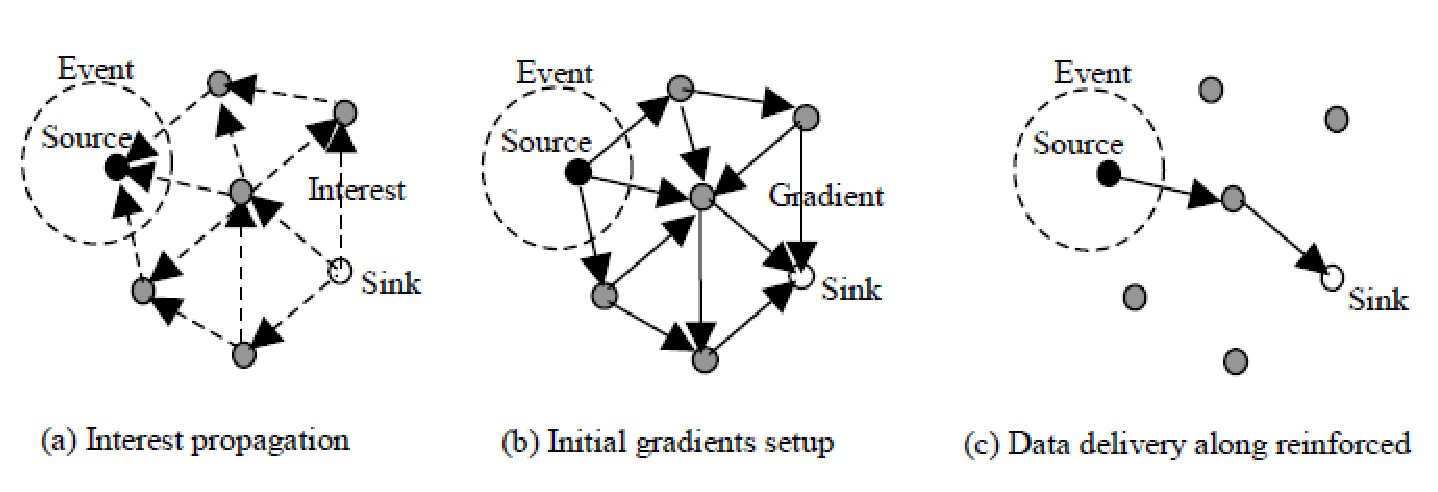
\includegraphics[width=\textwidth]{images/directed_diffusion.eps}
	\caption{Ένα σενάριο του πρωτοκόλλου Directed Diffusion.}
	\label{fig:dd_example}
\end{figure}

Το πρωτόκολλο Directed Diffusion διαφέρει από το SPIN ως προς το τρόπο που ζητάει τις πληροφορίες, δηλαδή τον τρόπο που θέτει τα επερωτήματα. Στο DD η πηγή θέτει
επερώτημα σε όλους τους αισθητήρες αν κάποια συγκεκριμένα δεδομένα είναι διαθέσιμα. Αν υπάρχουν τα δεδομένα ανάλογα με τα μονοπάτια που έχουν δημιουργηθεί, αυτά
ενισχύονται από την πηγή. Αντίθετα στο SPIN κάθε κόμβος διαφημίζει τα δεδομένα του στους υπόλοιπους κόμβους. Εαν κάποιος κόμβος ενδιαφέρεται τότε τα απαιτεί.Είναι
εμφανές οτι στο πρωτόκολλο DD υπάρχει υπεροχή όσον αφορά στην εξοικονόμηση ενέργειας ειδικά αν τα γεγονότα που εμφανίζονται στο δίκτυο έχουν μεγάλη διάρκεια. Όμως αν
τα γεγονότα έχουν πολύ μικρή διάρκεια τότε το DD έχει πολύ μικρή απόδοση αφού το \textbf{overhead} που θα υπάρχει μέχρι να στηθούν τα μονοπάτια θα είναι συγκρίσιμο με
την ενέργεια που σπαταλάται για να μεταφερθούν τα πραγματικά δεδομένα.

\paragraph{Rumor routing:} Η δρομολόγηση ανα φήμες (rumor routing) \cite{rumor_routing} είναι μια παραλλαγή του πρωτοκόλου Directed Diffusion και έχει κυρίως να κάνει
με ΑΔΑ στα οποία γεογραφικά κριτήρια δεν μπορούν να εφαρμοστούν. Γενικώς το DD πλημμυρίζει το δίκτυο με πακέτα προς όλους τους κόμβους μεχρι να φτιαχτούν τα
πραγματικά μονοπάτια τα οποία θα εμπεριέχουν ένα πολύ μικρό ποσοστό των συνολικών κόμβων του δικτύου. Αντίθετα στην δρομολόγηση ανα φήμες ο κάθε κόμβος προωθεί το
αναγνωριστικό πακέτο μόνο αν έχει "ακούσει" και ο ίδιος κάτι. Προσομοιώσεις έχουν δείξει οτι με αυτόν τον τρόπο εξοικονομείται περισσότερη ενέργεια στο δίκτυο
αισθητήρων μόνο όταν ο αριθμός των γεγονότων είναι σχετικά μικρός.

\paragraph{COUGAR:} Το αυτό δεδομενο-κεντρικό πρωτόκολλο είναι ριζοσπαστικό σε σχέση με τα υπόλοιπα καθώς βλέπει όλο το δίκτυο ως μια τεράστια, κατανεμημένα, βάση
δεδομένων \cite{cougar_protocol}. Η βασική ιδέα είναι να χρησιμοποιεί δηλωτικά ερωτήματα (declarative queries) με σκοπό να δημιουργήσει αφηρημένα επερωτήματα όπως η
επιλογή όλων των σχετικών κόμβων με μια πληροφορία κλπ. Αυτή η αφαίρεση γίνεται μέσα από ένα καινούργιο επίπεδο, αυτό των επερωτημάτων ανάμεσα στο επίπεδο δικτύου και
το επίπεδο των εφαρμογών. Όμως παρόλο που το επίπεδο αυτό είναι ανεξάρτητο του δικτύου έχει κάποια μειονεκτήματα. Κατ'αρχήν ένα επιπλέον επίπεδο στην στοίβα του
δικτύου θα καταναλώνει περισσότερη ενέργεια σε κάθε κόμβο. Επιπλέον, όπως και στις πραγματικές κατανεμημένες βάσεις δεδομένων, έτσι και εδώ θα πρέπει να λύνονται
αποδοτικά θέματα συγχρονισμού.

\subsection{Ιεραρχικά Πρωτόκολλα}
Όπως και στα κλασσικά δίκτυα ένα από τα πιο σημαντικά ζητήματα σχεδιασμού είναι αυτό της κλιμακωσιμότητας. Ένα "επίπεδο" δίκτυο μπορεί να προκαλέσει στην πύλη
δικτύου (gateway) υπερφόρτωση όταν το μέγεθος του δικτύου γίνει πολύ μεγάλο. Κατα συνέπεια η υπερφόρτωση μπορεί να προκαλέσει σοβαρή καθυστέρηση στις επικοινωνίες
και αντίστοιχα να χαθούν μερικά γεγονότα ή οι χρονικοί περιορισμοί που ορίζονται από αυτά. Ειδικά στην περίπτωση των ΑΔΑ όπου ο κάθε κόμβος έχει πολύ μικρή ακτίνα
εμβέλειας, η κλιμακωσιμότητα ενός "επίπεδου" πρωτοκόλλου δρομολόγησης είναι πολύ δύσκολη. Το πρόβλημα μπορεί να λυθεί εισάγοντας την έννοια της ιεραρχίας που πολλές
φορές γίνεται με μικρές συστάδες (clusters) σε όλη την περιοχή του δικτύου. Σε κάθε συστάδα συνήθως εκλέγεται ένας αρχηγός (cluster head) ο οποίος είναι υπεύθυνος για
την συστάδα του. Τα μέλη της συστάδας, κόμβοι του ΑΔΑ, ορίζονται από την ακτίνα εμβέλειας του αρχηγού όταν αυτός εκπέμψει ένα αναγνωριστικό μήνυμα. Αν σε έναν κόμβο
έρθει παραπάνω από ένα αναγνωριστικά μηνύματα τότε ο κόμβος θα γίνει μέλος της συστάδας της οποία το αναγνωριστικό σήμα είχε το καλύτερο (δυνατότερο) σήμα. Στην
συνέχεια παρουσιάζονται τα πιο γνωστά ιεραρχικά πρωτόκολλα δρομολόγησης.

\paragraph{LEACH:} Το πρωτόκολλο LEACH (Low-Energy Adaptive Clustering Hierarchy) \cite{leach_protocol} είναι ένα από τα πιο γνωστά ιεραρχικά πρωτόκολλα δρομολόγησης
για δίκτυα αισθητήρων. Η βασική ιδέα είναι να δημιουργηθούν συστάδες (clusters) βάση την ισχύ του ληφθέντος σήματος από τον αρχηγό. Οι κόμβοι της κάθε συστάδας,
χρησιμοποιώντας πολυ-βηματικές (multi-hop) μεταδόσεις, στέλνουν τα δεδομένα τους στον αρχηγό ο οποίος τα μαζεύει και τα στέλνει απευθείας στην πηγή. Με αυτόν τον
τρόπο μειώνεται η κατανάλωση της ενέργειας αφού μόνο οι αρχηγοί κάνουν μακρινές μεταδόσεις δεδομένων. Έχει υπολογιστεί οτι ο βέλτιστος αριθμός αρχηγών σε ένα δίκτυο
είναι περίπου το 5\% όλων των κόμβων του δικτύου. Προκειμένου να υπάρχει ακόμη μεγαλύτερη ισορροπία στην ενέργεια, οι αρχηγοί και κατα συνέπεια και οι συστάδες,
αλλάζουν ανα τακτά χρονικά διαστήματα. Συγκεκριμένα ένας κόμβος γίνεται αρχηγός με την παρακάτω πιθανότητα:

\begin{align*}
T(n) = \left\{
\begin{array}{cc}
 \frac{p}{1-p\cdot(r \text{mod}\frac{1}{p})} & \text{if } x<0 \\
  0 & \text{αλλιώς}
\end{array} \right.
\end{align*}
όπου $p$ είναι το επιθυμητό ποοστό των αρχηγών, $r$ είναι ο τρέχον γύρος και G είναι το σύνολο των κόμβων που δεν έχουν γίνει αρχηγοί τους προηγούμενους $\frac{1}{p}$
γύρους.

Το πρωτόκολλο LEACH μπορεί να πετύχει μέχρι και 7 φορές λιγότερη κατανάλωση ενέργειας σε σχέση με τα κλασσικά πρωτόκολλα ασύρματων δικτύων \cite{leach_protocol} ενώ
ακόμα και 12 χρόνια μετά την δημοσίευσή του παραμένει ένα από τα πιο κλασσικά πρωτόκολλα ΑΔΑ. Τα μόνα μειονεκτήματά του (τα οποία βελτιώθηκαν από επόμενες
δημοσιεύσεις) είναι οτι το μοντέλο που υποθέτει για την ακτίνα εμβέλειας των κόμβων, για πολύ μεγάλα δίκτυα, είναι μη ρεαλιστικό. Επίσης, για πολύ μεγάλα δίκτυα οι
αρχηγοί των συστάδων που βρίσκονται πολύ μακριά από την Πηγή εξαντλούν πολύ πιο γρήγορα την ενέργειά τους απ'ότι οι αρχηγοί των συστάδων που βρίσκονται κοντά στην
πηγή.

\paragraph{PEGASIS \& Hierarchical-PEGASIS:} Το πρωτόκολλο PEGASIS (Power-Efficient Gathering in Sensor Information Systems) \cite{pegasis_protocol} αποτελεί μια
βελτίωση του πρωτοκόλλου δρομολόγησης LEACH. Αντί να δημιουργούνται συστάδες, το PEGASIS σχηματίζει αλυσίδες με όλους τους κόμβους έτσι ώστε κάθε κόμβος λαμβάνει μόνο
από έναν κόμβο και αφού ενσωματώσει και τα δικά του δεδομένα τα αποστέλει σε μόνον έναν γείτονα. Ταυτόχρονα μόνο ένας κόμβος στην αλυσίδα έχει επιλεχτεί τυχαία ως
αρχηγός ο οποίος αναλαμβάνει να μαζέψει όλα τα δεδομένα και τα αποστέλει στην Πηγή. Η διαφορά από το LEACH είναι οτι χρησιμοποιεί πολυ-βηματικες (multi-hop)
μεταδόσεις μεταξύ των κόμβων και οτι μόνο ένας κόμβος σε κάθε γύρο είναι ο αρχηγός που αποστέλει τα δεδομένα στην Πηγή. Προσομοιώσεις δείξαν οτι μπορεί να βελτιώσει
ακόμα και 100\% την εξοικονόμηση ενέργειας σε σχέση με το LEACH. Το αρνητικό του όμως είναι οτι μπορεί τα πακέτα να έχουν μεγάλη καθυστέρηση μέχρι να φτάσουν στην
Πηγή. Το πρωτόκολλο Hierarchical-PEGASIS \cite{hierarchical_pegasis} αποτελεί μια προέκταση του PEGASIS το οποίο σκοπεύει στην μείωση της καθυστέρησης που
παρουσιάζεται στο PEGASIS. Ουσιαστικά δημιουργούνται περισσότερες από μια αλυσίδες με τον ίδιο προορισμό. Επίσης για την δημιουργία της αλυσίδας εφαρμοζει την μετρική
$energy\times delay$.

\paragraph{TEEN \& APTEEN:} Το πρωτόκολλο TEEN (The Energy Efficient sensor Network protocol) \cite{teen_protocol} είναι ένα
ιεραρχικό πρωτόκολο σχεδιασμένο να μπορεί να ανταποκρίνεται γρήγορα στις γρήγορες αλλαγές όπως είναι η θερμοκρασία με μεγάλη λεπτομέρεια. Η γρήγορη ανταπόκριση είναι
σημαντικό στοιχείο σε δίκτυα πραγματικού χρόνου. Οι συστάδες (clusters) σχηματίζονται παρόμοια με το LEACH πρωτόκολλο αλλά για για να πετύχει την γρήγορη ανταπόκριη,
το πρωτόκολλο ορίζει δύο κατώφλια που έχουν σχέση με τον τρόπο ανίχνευσης των γεγονότων από τους κόμβους. Το πρώτο ονομάζεται το σκληρό κατώφλι (hard threshold) και
ορίζει τις μικρότερες δυνατές τιμές μιας ιδιότητας που θα κάνουν τον κόμβο να "ξυπνήσει", δηλαδή να επανέλθει σε κανονική λειτουργία και να ενεργοποιήσει τον μεταδότη
του. Επομένως το σκληρό κατώφλι επιτρέπει τον κάθε κόμβο να αναφέρει δεδομένα μόνο όταν οι ιδιότητες αυτών ξεπεράσουν μια συγκεκριμένη τιμή που έχει να κάνει με το
πόσο ενδιαφέρον έχουν τα δεδομένα. Αντίθετα το μαλακό κατώφλι (soft threshold) επιτρέπει την μετάδοση δεδομένων μόνο όταν το ποσοστό των αλλαγών ξεπεράσουν την τιμή
του μαλακού κατωφλίου. Έτσι μειώνονται ακόμα περισσότερο οι μεταδόσεις πακέτων οι οποίες αφορούν πολύ μικρές αλλαγές στην περιοχή αίσθησης του κόμβου. Το μόνο
πρόβλημα που αντιμετωπίζει το πρωτόκολλο TEEN είναι όταν ο διαχειριστής του δικτύου επιθυμεί ο κάθε κόμβος να επιστρέφει πληροφορίες σε περιοδικό χρόνο. Το πρόβλημα
αυτό λύθηκε από μια προέκταση του TEEN, το ATEEN (Adaptive TEEN) \cite{apteen_protocol} στο οποίο μπορεί να ορίσει η πηγή με ποιον τρόπο θα γίνονται οι αναφορές από
κάθε κόμβο.


\subsection{Πρωτόκολλα Βασισμένα στην Τοποθεσία}
Πολλές φορές πρωτόκολλα για τα ΑΔΑ απαιτούν πληροφορίες για την τοποθεσία για τους κόμβους.
Στις περισσότερες περιπτώσεις οι πληροφορίες αυτές χρειάζονται για να υπολογιστούν οι αποστάσεις μεταξυ κόμβων και να εκτιμηθεί η ενέργεια που χρειάζεται για να
αποσταλή ένα πακέτο.
Επιπλέον, εφόσον δεν εφαρμόζονται πρωτόκολλα βασισμένα στην διευθυνσιοδότηση IP για τα δίκτυα αισθητήρων όπως συμβαίνει στα κλασσικά δίκτυα δεδομένων, ενώ ταυτόχρονα
οι κόμβοι είναι όλοι τοποθετημένοι σε μια συγκεκριμένη γεωγραφική περιοχή, πληροφορίες για την συγκεκριμένη τοποθεσία τους μέσα στην γεωγραφική περιοχή μπορούν
να χρησιμοποιηθούν για την δρομολόγηση δεδομένων και την μείωση της κατανάλωσης της ενέργειας.
Για παράδειγμα, αν η περιοχή που πρέπει να επιβλεφθεί για συγκεκριμένο σκοπό είναι γνωστή, χρησιμοποιώντας τις πληροφορίες τοποθεσίας των κόμβων, το επερώτημα (query)
προς το δίκτυο μπορεί να διοχετευθεί σε συγκεκριμένους κόμβους μόνο.
Αν και έχουν αναπτυχθεί αρκετά πρωτόκολλα τοπολογικής δρομολόγησης για τα κλασσικά ασύρματα δίκτυα αισθητήρων, αυτά δεν είναι εφαρμοσιμα στα ΑΔΑ καθώς η μετρική
απόδοσης που έχουν δεν περιλαμβάνει την μείωση της καταναλισκόμενης ενέργειας. Παρακάτω παρουσιάζονται τα πιο γνωστά πρωτόκολλα δρομολόγησης που βασίζονται στην
τοπολογία.


\paragraph{GAF:} Το πρωτόκολλο GAF (Geographic Adaptive Fidelity) \cite{gaf_protocol} είναι ένας ενεργειακός και βασισμένος στην τοπολογία αλγόριθμος δρομολόγησης
σχεδιασμένος αρχικά για ασύρματα δίκτυα αλλά πλέον εφαρμόζεται και σε ασύρματα δίκτυα αισθητήρων. Ο αλγόριθμος αυτός, εξοικονομεί ενέργεια απενεργοποιώντας περιττούς
κόμβους χωρίς να επηρεάζει την ποιότητα δρομολόγησης του δικτύου. Ο αλγόριθμος δημιουργεί ένα εικονικό πλέγμα (grid) για την περιοχή που καλύπτεται. Κάθε κόμβος
χρησιμοποιεί την τοποθεσία του για να συσχετίσει τον εαυτό του με κάποιο σημείο (τετράγωνο) του πλέγματος. Οι κόμβοι που είναι συσχετισμένοι με το ίδιο σημείο στο
πλέγμα θεωρούνται οτι είναι ισοδύναμοι όσον αφορά το κόστος της δρομολόγησης. Αυτή η ισοδυναμία εκμεταλεύεται απενεργοποιώντας μερικούς κόμβους και αφήνοντας μόνο
έναν ενεργοποιημένο σε κάθε σημείο (τετραγωνάκι) του πλέγματος. Ένα παράδειγμα φαίνεται στην εικόνα \ref{fig:gaf_example}. Συγκεκριμένα ο κόμβος 1 μπορεί να
επικοινωνήσει τους 2,3 και 4 και οι κόμβοι 2,3 και 4 μπορούν να επικοινωνήσουν με τον κόμβο 5. Επομένως οι κόμβοι 2,3 και 4 είναι ισοδύναμοι και οι δύο από αυτούς
μπορούν να απενεργοποιηθούν εξοικονομώντας ενέργεια.

\begin{figure}[h]
	\centering
	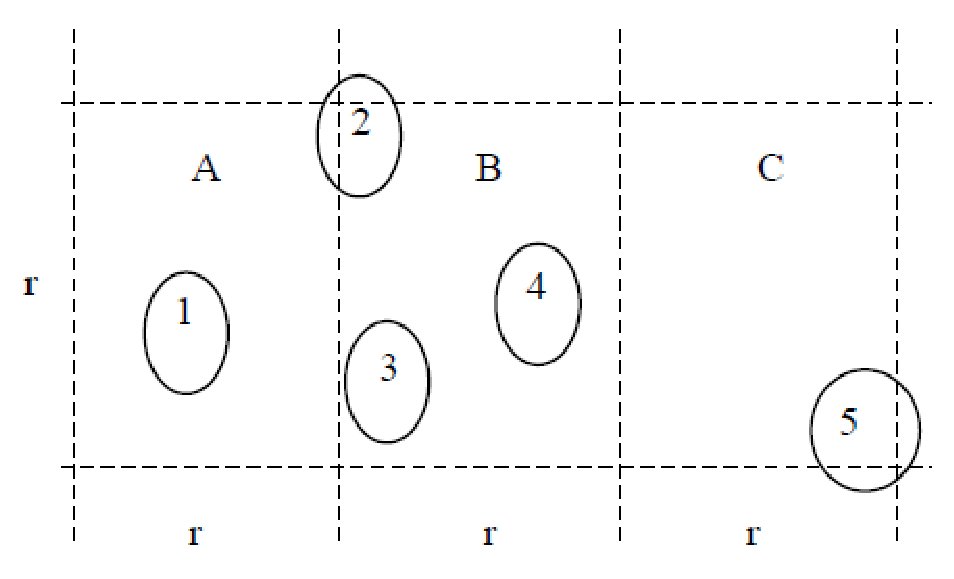
\includegraphics[width=0.6\textwidth]{images/gaf_example.eps}
	\caption{Ένα σενάριο του πρωτοκόλλου GAF.}
	\label{fig:gaf_example}
\end{figure}

Οι εξομοιώσεις έχουν δείξει οτι το πρωτόκολλο GAF μπορεί να έχει την ίδια απόδοση όσον αφορά την χρονοκαθυστέρηση (latency) και την απώλεια πακέτων σε σχέση με τα
κλασσικά πρωτόκολλα ασύρματων δικτύων, ενώ ταυτόχρονα αυξάνει την διάρκεια ζωής του δικτύου σε σημαντικό βαθμό.

\paragraph{GEAR: } Το πρωτόκολλο GEAR (Geographical and Energy Aware Routing) \cite{gear_protocol} προτείνει την χρησιμοποίηση γεγραφικών δεδομένων για την διάδοση
επερωτημάτων για συγκεκριμένες περιοχές αφού στις επερωτήσεις πολύ συχνά ενσωματώνονται γεωγραφικές ιδιότητηες. Το πρωτόκολλο χρησιμοποιεί ενεργιακές και γεωγραφικές
ευρετικές μεθόδους προκειμένου να δρομολογήσει κάποιο πακέτο. Η ιδέα είναι να περιορίσει τον αριθμό των πακέτων "ενδιαφέροντος" που χρησιμοποιεί το πρωτόκολλο
Directed Diffusion \cite{directed_diffusion} θεωρώντας μονο μια συγκεκριμένη περιοχή και όχι όλη την περιοχή του δικτύου. Στο πρωτόκολλο GEAR, κάθε κόμβος κρατάει
ένα κόστος εκτίμησης και ένα κόστος μάθησης της διαδρομής του πακέτου μέχρι τον προορισμό. Το κόστος εκτίμησης είναι ένας συνδυασμός την υπολοιπόμενης ενέργειας και
της απόστασης μέχρι τον προορισμό. Το κόστος μάθησης είναι ουσιαστικά το κόστος μάθησης αλλά λαμβάνει υπόψην και της ενεργειακές τρύπες του δικτύου που συμβαίνουν
όταν ένας κόμβος δεν έχει κανένα κοντινότερο γείτονα προς τον προορισμό εκτός από τον εαυτό του. Το κόστος μάθησης διαδίδεται ένα βήμα (hop) μακριά κάθε φορά που ένα
πακέτο φτάνει στον προορισμό του έτσι ώστε να χρησιμοποιηθεί στην επόμενη δρομολόγηση.


% \paragraph{GPSR:} Το πρωτόκολλο GPSR (Greedy Perimeter Stateless Routing for Wireless Networks)


\subsection{Πρωτόκολλα Εξισορόπισης Ενέργειας}
Όλα τα προηγούμενα πρωτόκολλα είχαν στόχο την μείωση της κατανάλωσης του δικτύου αισθητήρων και ως απώτερο σκοπό την επέκταση της διάρκειας ζωής του δικτύου.
Όμως πολλά από αυτά τα πρωτόκολλα δημιουργούν "παρενέργειες" σε ένα ΑΔΑ.
Για παράδειγμα στο πρωτόκολλο LEACH \cite{leach_protocol} οι αρχηγοί των συστάδων στέλνουν τα δεδομένα τους κατευθείαν στην πηγή. Όμως οι αρχηγοί των συστάδων οι
οποίες βρίσκονται στην άκρη του δικτύου, δηλαδή μακριά από την Πηγή έχουν πολύ μεγαλύτερο κόστος μετάδοσης από ότι οι αρχηγοί των συστάδων που βρίσονται κοντά στην
Πηγή.
Επομένως οι κόμβοι που βρίσκονται μακριά από την Πηγή εξαντλούν πολύ γρηγορότερα την ενέργειά τους και ενώ το δίκτυο συνεχίζει τη λειτουργία του, ένα κομμάτι
του δεν επιβλέπεται.
Ενα παρόμοιο παράδειγμα είναι το πρωτόκολλο Directed Diffusion \cite{directed_diffusion} όπου αφού φτιαχτούν τα μονοπάτια, δημιουργείται μια δενδρική δομή με ρίζα την
Πηγή όπου όλοι οι κόμβοι στέλνουν προς την Πηγή.
Είναι επομένως λογικό οτι οι κόμβοι που είναι κοντά στην Πηγή, αντιμετωπίζουν ένα πολύ μεγαλύτερο φορτίο σε σχέση με τους κόμβους που είναι μακρία από την αυτή.
Ένα παράδειγμα φαίνεται στην εικόνα \ref{fig:energy_holes}.

\begin{figure}[h]
	\centering
	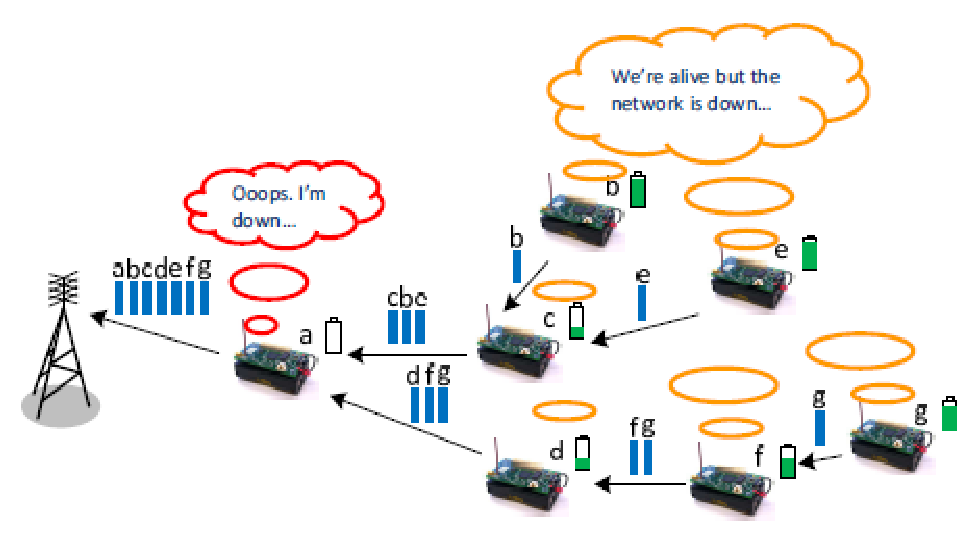
\includegraphics[width=0.8\textwidth]{images/energy_holes.eps}
	\caption{Ένα παράδειγμα υπερφόρτωσης των κόμβων κοντά στην Πηγή}
	\label{fig:energy_holes}
\end{figure}

Λόγω αυτής της υπερφόρτωσης των κόμβων κοντά στην πηγή, οι κόμβοι κοντά στην Πηγή αποφορτίζονται πολύ πιο γρήγορα από ότι οι κόμβοι μακριά από την
Πηγή. Έτσι μετά από μικρό χρονικό διάστημα λειτουργίας του δικτύου οι κόμβοι αυτοί πεθαίνουν και δημιουργούνται μικρές ενεργειακές τρύπες (energy holes). Αυτό
δημιουργεί πρόβλημα στο δίκτυο καθώς αν όλοι οι κόμβοι κοντά στην Πηγή αποφορτιστούν πλήρως, τότε ουσιαστικά το δικτυο καθίσταται άχρηστο καθώς οι κόμβοι που είναι
λίγο πιο μακριά από την Πηγή δεν μπορούν να στείλουν τα δεδομένα τους σε αυτήν. Μάλιστα, έχει δειχθεί οτι σε πρωτόκολλα όπως το Directed Diffusion όταν οι κομβοί
κοντά στην Πηγή πεθάνουν, το δίκτυο έχει ακόμα το 90\% της ενέργειας του \cite{energy_holes}, όπου το μεγαλύτερο μέρος αυτής είναι κατανεμημένο στους κόμβους που
βρίσκονται στην άκρη του δικτύου. Αυτό σημαίνει οτι δεν υπάρχει αποδοτική διαχείρηση της ενέργειας σε αυτά τα πρωτόκολλα. Η λύση σε αυτό το πρόβλημα δίνεται από
αλγόριθμους εξισορρόπησης ενέργειας.

Τα πρωτόκολλα εξισσορόπησης ενέργειας αυτό που προσπαθούν να κάνουν είναι, σε κάθε χρονική στιγμή, όλοι οι κόμβοι του δικτύου να έχουν περίπου την ίδια ενέργεια.
Είναι προφανές οτι τα πρωτόκολλα εξισορρόπησης ενέργειας καταναλώνουν περισσότερη ενέργεια από ότι τα πρωτόκολλα μείωσης της κατανάλωσης ενέργειας. Όμως η διαρκεια
ζωής\footnote{διάρκεια ζωής εννοούμε το χρονικό διάστημα μέχρι το δίκτυο να γίνει άχρηστο.} ενός ΑΔΑ αυξάνεται σημαντικά με τα πρωτόκολλα εξισορρόπησης ενέργειας
αφού σχεδόν όλοι οι κόμβοι είναι ενεργοί καθόλη τη διάρκεια της ζωής του δικτύου ενώ πεθαίνουν όλοι σχεδόν ταυτόχρονα προς το τέλος της. Υπάρχει πoλύ μεγάλη έρευνα
για την εξισορρόπηση ενέργειας στα ασύρματα δίκτυα αισθητήρων ακόμα και σήμερα. Τα πιο σημαντικά πρωτόκολλα
εξισορρόπησης ενέργειας παρουσιάζονται παρακάτω:

\paragraph{EBP:} Το πρωτόκολλο EBP (Energy Balanced Protocol) \cite{ebp_protocol} είναι από τα πρώτα πρωτόκολλα εξισορρόπησης ενέργειας το οποίο έθεσε τις βάσεις του
προβλήματος και πρότεινε έναν πιθανοτικό αλγόριθμο. Συγκεκριμένα, το δίκτυο χωρίζεται σε $n$ δακτύλιους (ή τομείς), πλάτους $R$ ενώ η γωνία που καλύπτει το δίκτυο
θεωρείται οτι είναι $\phi$ οπως φαίνεται στην εικόνα \ref{fig:ebp_ring}.

\begin{figure}[h]
	\centering
	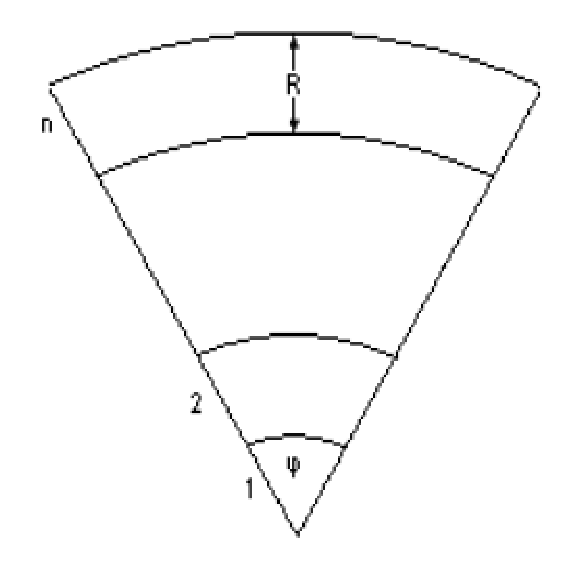
\includegraphics[width=0.4\textwidth]{images/ebp_ring.eps}
	\caption{Δίκτυο αισθητήρων με $n$ δακτυλίδια, γωνία $\phi$ και πλάτος δακτύλιου $R$}
	\label{fig:ebp_ring}
\end{figure}

Για την μετάδοση των πακέτων κάθε κόμβος στον δακτύλιο $i$ χρησιμοποιείται το εξής σχήμα:
\begin{itemize}
\item Μετάδοσε το πακέτο στον δακτύλιο $i-1$ με πιθανότητα $p_{i}$
\item Μετάδοσε το πακέτο απευθείας στην πηγή με πιθανότητα $1-p_{i}$
\end{itemize}

Η επιλογή του $p_{i}$ γίνεται με τέτοιο τρόπο ώστε η μέση κατανάλωση ενέργειας κόμβου να είναι ίδια για όλους τους κόμβους στο δίκτυο.
Μετά από μία εκτενή ανάλυση οι συγγραφείς καταλήγουν στον παρακάτω τύπο:
\begin{align*}
p_{i} = \frac{E[f_{i}]}{E[f_{i+1}] + E[g_{i+1}]}
\end{align*}
όπου $E[f_{i}]$ είναι η μέση τιμή των μηνυμάτων που προωθούνται στον δακτύλιο $i$ και
\begin{align*}
E[f_{i}] = - \sum\limits^{n-i}_{k=1}\frac{\prod_{j=k}^{n-i+1}\alpha(n-j)}{\prod_{j=k}^{n-i}d(n-j)}\cdot
\left(\sum\limits_{j=1}^{n-k}(a(j)E[g_{j}]-\alpha(j+1)E[g_{j+1}])+\alpha(1)\cdot E[f_{1}]\right)
\end{align*}
ενώ $E[g_{i}]$ η μέση τιμή των μηνυμάτων που παράγονται και καθορίζονται από το δίκτυο.

Κάνοντας την παραδοχή οτι $E[f_{i}] \approx E[f_{i+1}]$, οτι δηλαδή τα μηνύματα που προωθούνται στον δακτύλιο $i$ είναι περίπου ίσα με τα μηνύματα που προωθούνται
στον δακτύλιο $i+1$ τότε δημιουργείται ο εξής κλειστός προσεγγιστικός τύπος για τις πιθανότητες $p_{i}$:
\begin{align*}
p_{i} = \frac{3x}{(i+1)(i-1)}
\end{align*}
όπου $p_{2} = x \in (0,1)$ είναι παραμετροποιήσιμη μεταβλητή ενώ $p_{1} =0$.

Όταν το $i$ είναι μεγάλο τότε και η πιθανότητα $p_{i}$ είναι μεγάλη. Αυτό συμβαίνει γιατί όταν ένας κόμβος είναι μακριά από το sink τότε είναι
καλύτερα να στέλνει hop by hop για να αποφύγει να σπαταλήσει μεγάλη ενέργεια για την αποστολή απευθείας στην Πηγή. Αντίθετα, όταν το $i$ είναι μικρό τότε η
πιθανότητα $p_{i}$ είναι μικρή.

\paragraph{Distributed EBP} Η εργασία στο \cite{debp_protocol} είναι μια επέκταση του πρωτοκόλλου EBP. Αρχικά
ορίζεται ως μικτή στρατιγική την δυνατότητα κάθε κόμβου να μπορεί να στείλει είτε στον αμέσως επόμενο γείτονά του είστε απευθείας στην πηγή όπως στο EBP.
Αποδεικνύεται οτι οι μικτές στρατηγικές είναι οι βέλτιστες σε σχέση με οποιαδήποτε άλλη στρατηγική μετάδοσης των πακέτων. Στην συνέχεια κατασκευάζεται ένα τυφλό
άμεσης απόκρισης κατανεμημένο αλγόριθμο (blind, online distributed algorithm) ο οποίος λύνει το πρόβλημα της εξισορρόπησης της ενέργειας. Ο αλγόριθμος λειτουργεί ως
εξής:
\begin{itemize}
\item Αρχικά κάθε κόμβος ξέρει όλους τους γείτονές του και την εναπομείνουσα ενέργειά τους
\item Κάθε κόμβος που θέλει να στείλει ένα πακέτο βρίσκει τον γείτονα με την χαμηλότερη εναπομείνουσα ενέργεια έστω $n_{l}$
	\begin{itemize}
	\item Αν η εναπομείνουσα ενέργεια του $n_{l}$ είναι μεγαλύτερη από την εναπομείνουσα ενέργεια του κόμβου που θέλεί να στείλει το πακέτο τότε το στέλνει στον
$n_{l}$
	\item Αντίθετα αν η εναπομείνουσα ενέργεια του $n_{l}$ είναι μικρότερη τότε ο κόμβος που θέλει να στείλει το πακέτο το στέλνει απευθείας στην πηγή
	\end{itemize}
\end{itemize}

Όπως φαίνεται ο αλγόριθμος χρησιμοποιεί μικτή στρατιγική όπως ο EBP, αλλά είναι κατανεμημένος και χρησιμοποιεί μόνο τοπική πληροφορία, σε αντίθεση με τον EBP.
Εξομοιώσεις δείξαν οτι ο αλγόριθμος μπορεί να εξισορροπήσει σχεδόν τέλεια την ενέργεια σε ένα ασύρματο δίκτυο αισθητήρων.

\paragraph{Offline EBP} H εργασίες στα \cite{oebp_protocol1} και \cite{oebp_protocol2} προσπαθουν να λύσουν το πρόβλημα της εξισορρόπησης ενέργειας από μια
διαφορετική σκοπιά. Η πρώτη εργασία εξετάζει την περίπτωση ομοιόμορφης κατανομής των κόμβων σε ένα δίκτυο το οποίο είναι χωρισμένο σε δακτυλίους όταν ο κάθε κόμβος
στέλνει σχεδόν τον ίδιο αριθμό πακέτων στην Πηγή. Αρχικά αποδεικνύεται οτι για να μειωθεί στο ελάχιστο η κατανάλωση της ενέργειας, οι δακτύλιοι θα πρέπει να έχουν το
ίδιο πλάτος. Όμως με αυτόν τον τρόπο δημιουργείται ανισόρροπη κατανομή ενέργειας στο δίκτυο. Αντίθετα, αποδεικνύεται, οτι για να υπάρχει εξισορρόπηση ενέργειας, το
πλάτος των δακτυλίων μικραίνει όσο είναι πιο κοντά στην πηγή. Στην δεύτερη εργασία μελετάται το ίδιο πρόβλημα όταν υπάρχει μη ομοιόμορφη κατανομή των κόμβων μέσα στο
δίκτυο. Αποδυκνύεται οτι η ανομοιόμορφη κατανάλωση ενέργειας είναι μη αναπόφευκτη σε τέτοια είδη δικτύου. Οι συγγραφείς προτείνουν μία υποβέλτιστη λύση στην οποία ο
αριθμός των κόμβων αυξάνεται με γεωμετρικό ρυθμό από τος έξωτερικούς δακτυλίους προς του εσωετρικούς.


\section{Πρωτόκολλα Δρομολόγησης με Κινητούς Κόμβους}
Πρόσφατη έρευνα έχει δείξει οτι μπορεί να υπάρξει σημαντική μείωση στην κατανάλωση της ενέργειας αν μέσα στο δίκτυο αισθητήρων υπάρχουν μικρές μηχανικά κινητές
συσκευές, ή κινητή κόμβοι, οι οποίες είναι ικανές να μεταφέρουν δεδομένα από ένα σημείο σε ένα άλλο με μηχανική ενέργεια. Για παράδειγμα ένας κινητός κόμβος ο οποίος
μπορεί να μετακινείται μέσα σε όλο την περιοχή του δικτύου, πλησιάζει τους κόμβους αρκετά κοντά προκειμένου οι τελευταίοι να του στείλουν τα δεδομένα τους χωρίς
ιδιαίτερο κόστος. Στην συνέχεια, ο κινητός κόμβος συνεχίζει την πορεία του πλησιάζοντας και άλλους κόμβους για τον ίδιο λόγο. Ανά τακτά χρονικά διαστήματα, ο
κινητός κόμβος, επιστρέφει στην Πηγή πρεοκειμένου να παραδώσει τα δεδομένα του. Πιο ισχυρά μοντέλα υποθέτουν οτι ο κόμβος μπορεί να αποστείλει τα δεδομένα που κατέχει
στην Πηγή από οποιοδήποτε σημείο του δικτύου και αν βρίσκεται. Άλλα μοντέλα θεωρούν οτι η ίδια η πηγή είναι ο κινητός κόμβος. Επίσης στα περισσότερα μοντέλα, η
ενέργεια που καταναλώνει ο κινητός κόμβος κατα την κίνησή του δεν εξετάζεται και θεωρείται αμεληταία.

Ωστόσο, αυτή η αρχιτεκτονική σε κάποια ΑΔΑ μπορεί να δημιουργήσει προβλήματα, κυρίως θέματα χρονοκαθυστέρησης(delay). Για παράδειγμα, μια τυπική ταχύτητα για πολλούς
κινητούς κόμβους (για παράδειγμα το NIMs \cite{nims_mobile}, το Packbot\cite{dynamic_deadlines} και το Robomore\cite{robomore_mobile}) είναι περίπου $0.1-1m/s$.
Επομένως, θα χρειαστεί περίπου 15 λεπτά για μια κινητή συσκευή να διανύσει $1Km$ για να μαζέψει τις πληροφορίες. Τέτοιο χρόνοι είναι απαγορευτικοί για μερικά δίκτυα
αισθητήρων τα οποία απαιτούν πραγματικού χρόνου συλλογή δεδομένων. Σε μερικές εφαρμογές ΑΔΑ όπως είναι η διαχείρηση καταστροφών οι κινητοί κόμβοι θα μπορούσαν να
μεταφερθούν και από μη επανδρωμένα μικρά αεροσκάφη \cite{uav_mobile}. Οι τύποι των διαδρομών που ακολουθούν οι κινητοί κόμβοι μπορούν να ταξινομηθούν στις εξής 3
κατηγορίες:

\begin{itemize}
\item \textbf{Τυχαία κίνηση:} Μπορεί να επιτευχθεί όταν για παράδειγμα οι κόμβοι ενσωματωθούν σε ανθρώπους ή σε ζώα \cite{zebranet}. Γενικώς οι τυχαίοι περίπατοι
(random walks) έχει παρατηρηθεί οτι έχουν ούτε καλή αλλά ούτε κακή απόδοση, είναι όμως πάρα πολύ εύκολο να υλοποιηθούν.

\item \textbf{Ντετερμινιστική κίνηση:} Είδος κίνησης η τροχιά της οποίας είναι προδιαγεγραμμένη από την έναρξη λειτουργίας του δικτύου, όπως είναι ο κύκλος ή η
σπείρα. Οι ιδιότητες της κίνησης, όπως π.χ. ακτίνα, εξάγονται από το ίδιο το δίκτυο. Τέτοιες κινήσεις μπορούν να επιτευχθούν όταν για παράδειγμα οι κόμβοι
ενσωματωθούν σε ένα λεωφορείο το οποίο κάνει συνεχώς την ίδια διαδρομή. Το πλεονέκτημα αυτής της κίνησης είναι οτι αν είναι γνωστή στους στατικούς κόμβους, αυτοί
μπορούν να "ξυπνήσουν" την κατάλληλη στιγμή ωστε να στείλουν τα δεδομένα τους στον κινητό κόμβο.

\item \textbf{Προσαρμοστική κίνηση:} Αυτή η κίνηση εφαρμόζει τεχνικές αλγορίθμων μάθησης και τροποποιείται κατάλληλα ώστε να ανταποκρίνεται κάθε στιγμή στις
απαιτήσεις του δικτύου. Για παράδειγμα σε αν ένα σημείο του δικτύου υπάρχει πολύ μεγάλος ρυθμός παραγωγής γεγονότων, τότε ο κινητός κόμβος κάθεται για περισσότερο
διάστημα σε αυτό το σημείο ώστε να ξεκουράσει τους γύρω κόμβους.

\item \textbf{Ελεγχόμενη κίνηση:} Όταν ο κιητός κόμβος ενσωματωθεί σε ένα τηλεκατευθυνόμενο robot ή αεροπλάνο (UAV) τότε η κατεύθυνση και η ταχύτητα μπορεί να
τροποποιηθεί κάθε στιγμή από τον ίδιο τον άνθρωπο. Συνήθως τέτοιες κινήσεις δεν αναλύονται στα μοντέλα ΑΔΑ.
\end{itemize}



Γενικώς η κίνηση (είτε είναι κινητή Πηγή είτε κινητός κόμβος είτε πολλοί κινητοί κόμβοι) στα σύρματα δίκτυα αισθητήρων χρησιμοποιείται εξής λόγους:

\begin{itemize}
\item \textbf{Βελτίωση της κάλυψης του δικτύου:} Οι κόμβοι συνήθως αναπτύσσονται τυχαία μέσα στην περιοχή ανίχνευσης είτε από τον αέρα (π.χ. από ένα
αεροπλάνο/ελικόπτερο) είτε από ένα ρομπότ. Όμως ακόμα και αν θεωρηθεί οτι οι κόμβοι αναπτύσσονται ομοιόμορφα κατανεμημένα, αυτό δεν μπορεί να εγγυηθεί οτι δεν θα
υπάρχουν τοπικά μέγιστα και ελάχιστα. Επομένως μπορεί σε κάποιο σημείο του δικτύου να μην καλύπτεται επαρκώς από τους ήδη υπάρχοντες κόμβους. Ένας κινητός κόμβος
μπορεί να πάει σε αυτή τη θέση και να προσομοιώσει έναν στατικό κόμβο προκειμένου να καλυφθεί πλήρως η περιοχή ανίχνευσης.
\item \textbf{Βελτίωση της συνδεσιμότητας του δικτύου:} Οι κινητοί κόμβοι μπορούν να προσφέρουν ένα μονοπάτι ανάμεσα σε δύο συνεκτικές συνιστώσες του δικτύου. Για
παράδειγμα μπορεί μερικοί κρίσιμοι κόμβοι να πάθουν βλαβη και επομένως το δίκτυο να "κοπεί" ουσιαστικά στη μέση. Οι κινητοί κόμβοι μπορούν να αποτρέψουν ένα τέτοιο
γεγονός.
\item \textbf{Μεταφορά δεδομένων από απομακρυσμένους κόμβους:} Μερικοί κόμβοι σε ένα ασύρματο δίκτυο αισθητήρων μπορεί να μην έχουν συνδεσιμότητα με κανέναν άλλο
κόμβο και επομένως να μην μπορούν να μεταδώσουν τα δεδομένα τους στην Πηγή. Αυτό μπορεί να επιτευχθεί αν ένας κινητός κόμβος προσεγγίσει τους απομακρυσμένους κόμβους
της πηγής και λάβει τα αποθηκευμενα δεδομένα των κόμβων αυτών και τα μεταφέρει σε άλλους κόμβους ή στην Πηγή.
\item \textbf{Αύξηση του χρόνου ζωής του δικτύου:} Αποτελεί από τους πιο σημαντικούς λόγους που χρησιμοποιείται η κίνηση στα δίκτυα αισθητήρων. Οι κινητοί κόμβοι
μπορούν να προσεγγίσουν περιοχές στις οποίες υπάρχουν ενεργά μονοπάτια μεταφοράς δεδομένων και να βοηθήσουν αυτούς τους κόμβους μεταφέροντας οι ίδιοι τα δεδομένα
μηχνανικά.
\begin{figure}[h]
	\centering
	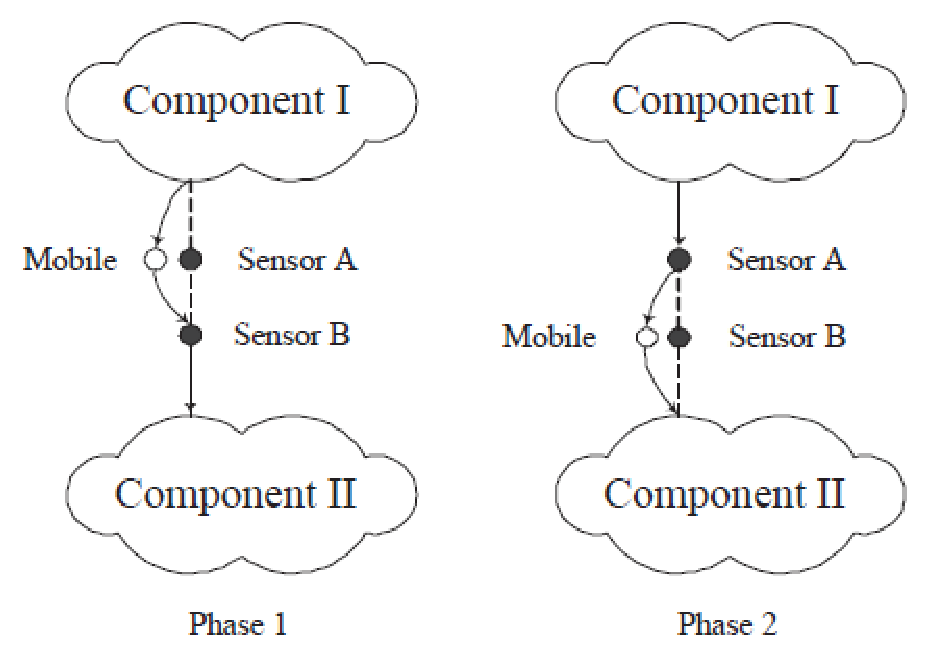
\includegraphics[width=0.6\textwidth]{images/mobile_help.eps}
	\caption{O κινητός κόμβος βοηθάει τους υπερφορτωμένους στατικούς κόμβους.}
	\label{fig:mobile_help}
\end{figure}
Ενα τέτοιο παράδειγμα φαίνεται στην εικόνα \ref{fig:mobile_help} (εξαγμένη από το \cite{using_mobile_elements_to_prolong_lefetime}). Ολόκληρο το δίκτυο αποτελείται
από δύο μικρότερα υποδύκτια ( Compnent I \& II) τα οποία είναι συνδεδεμένα μέσω των κόμβων Α και Β. Επομένως οι δύο αυτοί κόμβοι αποτελούν πέρασμα συμφώρησης αφού
πρέπει να προωθούν όλη την κίνηση από τα 2 υποδίκτυα. Ένας κινητός κόμβος μπορεί να προσομοιώσει την λειτουργία των Α και Β και έτσι να βελτιώσει τον χρόνο ζωής των
κόμβων αυτών και κατα συνέπεια του συνολικού δικτύου. Επίσης οι κινητοί κόμβοι μπορούν να συλλέξουν τα δεδομένα των στατικών κόμβων μέσω μικρής ακτίνα μετάδοσης
βοηθώντας στην εξοικονόμηση ενέργειας του κάθε κόμβου ξεχωιριστά. Συγκεκριμένα, προκειμένου να μεγιστοποιηθεί ο χρόνος ζωής στο δίκτυο, ο κάθε στατικός κόμβος θα
πρέπει να στέλνει τα δεδομένα του σε έναν κινητό κόμβο αν και μόνο αν αυτός είναι σε απόσταση μικρότερης του ενός βήματος (hop). Ωστόσο, με αυτόν τον τρόπο υπάρχει
πολύ μεγάλη χρονοκαθυστέρηση (delay) στην μεταφορά των δεδομένων στην Πηγή. Από την άλλη μεριά αποστέλοντας απ'ευθείας στην Πηγή ή χρησιμοποιώντας multi-hop
πρωτόκολλα για την άμεση αναφορά γεγονότων στην Πηγή μειώνει δραστικά την χρονοκαθυστέρηση αλλά και τον χρόνο ζωής του δικτύου. Επομένως απαιτείται μία χρυσή τομή
ανάμεσα στην χρονοκαθυστέρηση και τον χρόνο ζωής του δικτύου που σίγουρα εξαρτάται από τον σκοπό και το περιβάλλον του δικτύου αισθητήρων.
\end{itemize}

Στη βιβλιογραφία έχουν χρησιμοποιηθεί πολλές διαφορετικές έννοιες για την περιγραφή των κινητών κόμβων στα ασύρματα δίκτυα αισθητήρων. Οι όροι διαφέρουν μεταξύ τους
ως προς το είδος και τον σκοπό του κινητού κόμβου. Για παράδειγμα κινητή Πηγή (mobile Sink ή mobile BS) χρησιμοποιείται για να περιγράψει μια κινητή Πηγή η οποία
έχει την δυνατότητα να περισυλλέγει δεδομένα από τους κοντινούς της κόμβους καθώς κινείται προκειμένου αυτοί να κάνουν πιο εικονομικές μεταδόσεις σε σχέση με μία
στατική Πηγή. Παρόμοια ο όρος κινητή οντότητα ή πιο γενικά κινητός κόμβος (mobile MULES, mobile entities, mobile relays) αναφέρεται σε κινητούς κόμβους οι οποίοι
έχουν πρόμοια υπολογιστική ισχύ όπως μια Πηγή και περιφέρονται σε όλο την περιοχή προκειμένου να περισυλλέξουν δεδομένα. Συχνά σε αυτό το μοντέλο είναι οτι
στο ασύρματο δίκτυο υπάρχει και μία Πηγή στην οποία οι κινητοί κόμβοι στέλνουν τα δεδομένα των στατικών κόμβων.

Επειδή η έρευνα σε αυτό τον τομέα των ασύρματων δικτύων αισθητήρων συνεχίζεται ακόμα και υπάρχει μεγάλο ενδιαφέρον στην πλήρη αξιοποίηση των κινητών κόμβων σε ένα
ΑΔΑ, θα παρουσιαστούν παρακάτων οι πιο σημαντικές εργασίες σε σχέση με την εκμετάλευση κινητών Πηγών και κινητών κόμβων σε ένα δίκτυο αισθητήρων.

\subsection{Πρωτόκολλα με Κινητή Πηγή}
Η εργασία στο \cite{jointmobility} εξετάζει αν η κίνηση και η δρομολόγηση σε ένα δίκτυο αισθητήρων είναι φιλικές ή αλληλοσυγκρουόμενες έννοιες. Στο μοντέλο τους
εξετάζουν την περίπτωση ενός πυκνού δικτύου στο οποίο υπάρχουν στατικοί κόμβοι, τοποθετημένοι με μια Poisson κατανομή σε έναν κύκλο, έχουν μικρή ενέργεια και μια
κινητή Πηγή με άπειρη ενέργεια περιφέρεται στο δίκτυο προκειμένου να βοηθήσει στην δρομολόγηση και να περισυλλέξει τα δεδομένα όπως φαίνεται στην εικόνα
\ref{fig:jointmobility_model}.
\begin{figure}[h]
	\centering
	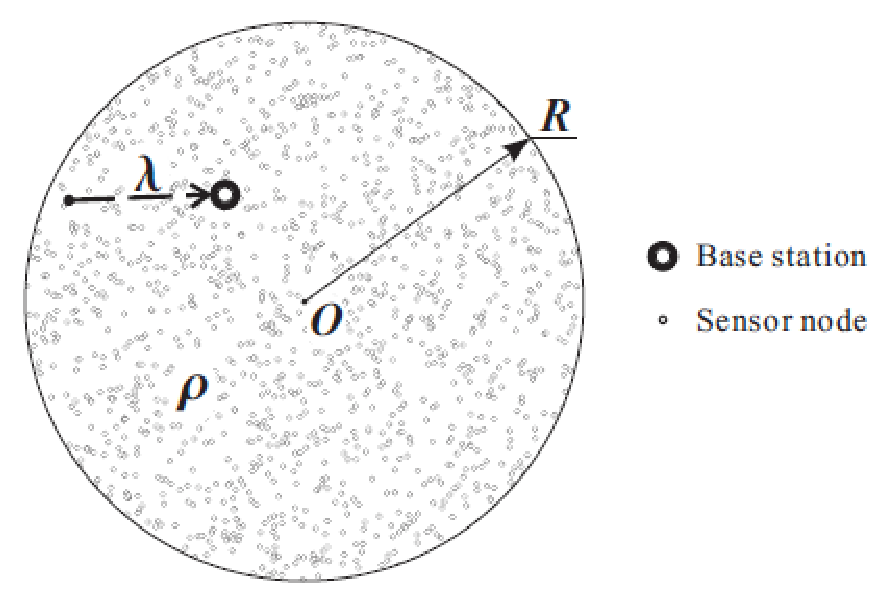
\includegraphics[width=0.6\textwidth]{images/jointmobility_model.eps}
	\caption{Κόμβοι τοποθετημένοι με Poisson κατανομή και Πηγή να κινειται στην περιφέρεια του κύκλου.}
	\label{fig:jointmobility_model}
\end{figure}
Οι συγγραφείς εξετάζουν την βέλτιστη θέση της Πηγής όταν αυτή είναι στατική και την βέλτιστη διαδρομή όταν αυτή είναι κινητή. Τελικά αποδεικνύουν οτι η βέλτιστη θέση
για την Πηγή όταν αυτή είναι στατική είναι το κέντρο του κύκλου. Αντίθετα όταν η Πηγή είναι κινητή αποδεικνύουν οτι η βέλτιστη διαδρομή της Πηγής είναι η περιφέρεια
του κύκλου. Αυτό συμβαίνει γιατί η διαδρομή αυτή είναι η μεγαλύτερη δυνατή που υπακούει και στην γεωμετρία του μοντέλου. Μια σύγκριση της εναπομείνουσας ενέργειας με
τα προαναφερθέντα μοντέλα φαίνονται στην εικόνα \ref{fig:jointmobility_dissipation}.
\begin{figure}[h]
	\centering
	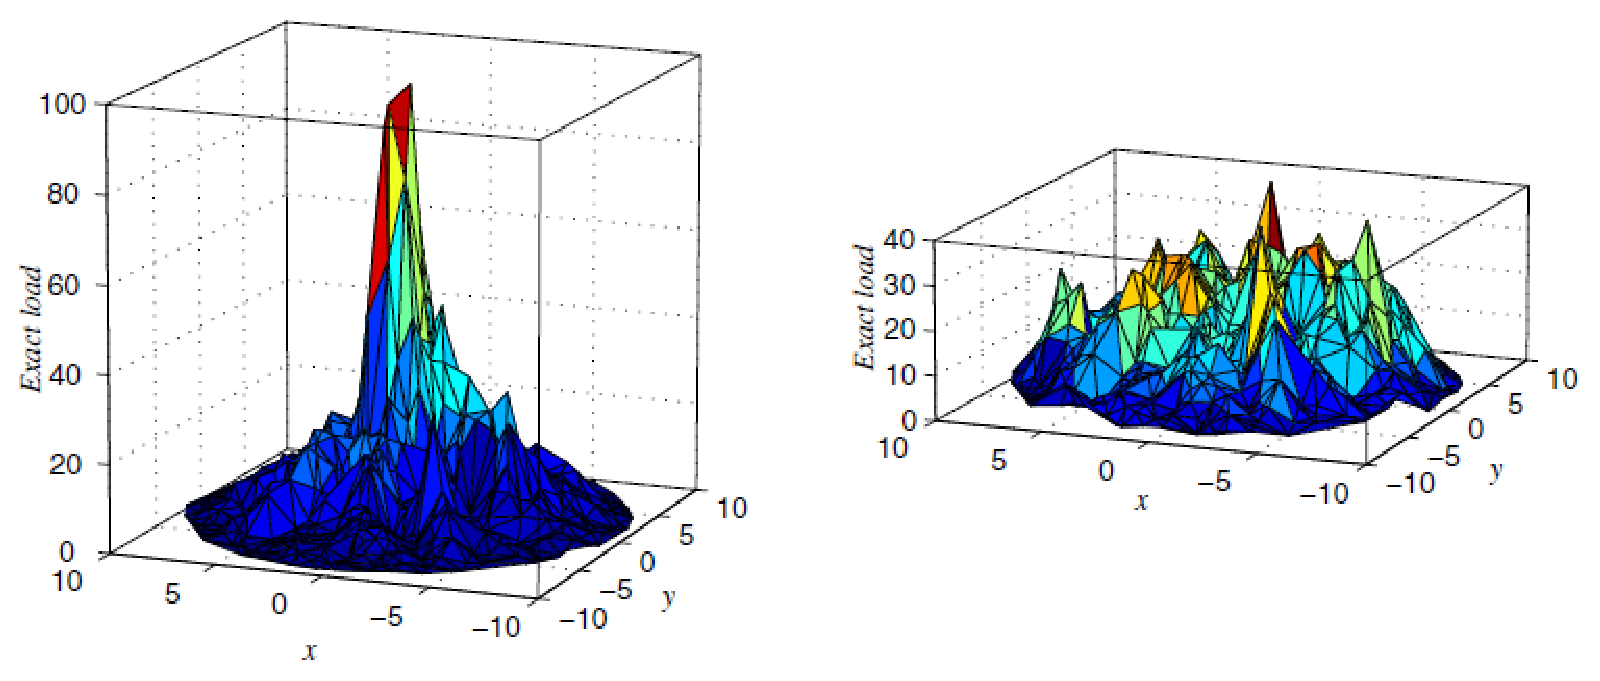
\includegraphics[width=\textwidth]{images/jointmobility_dissipation.eps}
	\caption{Ο ρυθμός κατανάλωσης της ενέργειας όταν η Πηγή είναι στο κέντρο του δικτύου(δεξιά) και όταν η κινείται στην περιφέρειά του(αριστερά).}
	\label{fig:jointmobility_dissipation}
\end{figure}

Όπως φαίνεται στην πρώτη εικόνα η στατική πηγή δημιουργεί στους γύρω της κόμβους πολύ μεγάλους ρυθμούς κατανάλωσης ενέργειας. Αντίθετα, όταν η Πηγή είναι κινητή και
κινείται στην περιφέρεια του κύκλου, υπάρχει μεγαλύτερη εξισσορόπηση ενέργειας στο δίκτυο και επομένως αυξάνεται ο χρόνος ζωής του.
\begin{comment}
edw den einai pio logiko h phgh na kineitai kapou sto endiameso ths aktinas R kai pio sugkekrimena otan ta 2 emvada ginoun isa ? prepei na to melethsw....
\end{comment}

Οι συγγραφείς παρουσίασαν μια ακόμη εργασία στο \cite{jointmobility_2006} ως συνέχεια της προηγούμενης στην οποία το μοντέλο με την προηγούμενη
εργασία και συγκρίνουν 2 περιπτώσεις για την αύξηση του χρόνου ζωής του δικτύου.
\begin{itemize}
\item \textbf{Γρήγορη κίνηση της Πηγής:} εξισσορόπηση της χρονοκαθυστέρησης (delay) με την κατανάλωση της ενέργειας
\item \textbf{Αργή κίνηση της Πηγής:} παροχή βοήθειας στους κρίσιμους κόμβους (bottleneck nodes)
\end{itemize}
Η αργή κίνηση της Πηγής επιτυγχάνεται μέσα από ένα γραμμικό πρόγραμμα
\begin{align*}
\text{Maximizing network lifetime } & T=\sum\limits_{i}T_{i}\\
\text{Constraints } & \sum\limits_{i}T_{i}P_{i}\leq E
\end{align*}
όπου $Τ_{i}$ ο χρόνος ζωής κάθε κόμβου, $P_{i}$ ο ρυθμός κατανάλωσης ενέργειας του κάθε κόμβου ως προς τον χρόνο και $E$ η συνολική ενέργεια του δικτύου.
Στην εργασία προτείνεται ένας αλγόριθμος 2 φάσεων ο οποίος χρησιμοποιεί το παραπάνω γραμμικό πρόγραμμα
\begin{itemize}
\item \textbf{Αρχικοποίηση:} Κατα την αρχικοποίηση η κινιτή Πηγή επισκέπτεται όλους τα σημεία-σταθμούς, συλλέγει τον ρυθμό κατανάλωσης κάθε σταθμού και κατασκευάζει
ένα προφίλ αυτού του σημείου-σταθμούς
\item \textbf{Εν λειτουργία:} Κατα την πραγματική λειτουργία η κινητή Πηγή παραμένει σε κάθε σημείο-σταθμό χρονικό διάστημα ανάλογο με τον ρυθμό κατανάλωσης ενέργειά
του.
\end{itemize}
Τα πειράματα αυτής της εργασίας έδειξαν οτι υπάρχει σημαντική αύξηση του χρόνου ζωής με τον αλγόριθμο των 2 φάσεων. Όμως ο αλγόριθμος δεν μπορεί να είναι
αποδοτικός και να επεκταθεί σε πολύ μεγάλα δίκτυα καθώς υπάρχει σημαντική καθυστέρηση.


Στην εργασία \cite{marios_randomwalks_1} αναλύεται η περίπτωση που υπάρχει κινητή Πηγή και αυτή κάνει έναν τυχαίο περίπατο (random walk). Γενικώς οι τυχαίοι
περίπατοι είναι πολύ εύκολοι στην υλοποίηση αφού χρησιμοποιούν μόνο τοπικές πληροφορίες και μπορούν να μειώσουν σημαντικά την κατανάλωση της ενέργειας λόγω της
τυχαιότητάς τους. Οι συγγραφείς προκειμένου να κάνουν ακόμα πιο αποδοτικούς τους τυχαίους περίπατους, δημιουργούν τους προσαρμοστικούς τυχαίους περίπατους. Σε αυτή
την περίπτωση, η κινητή Πηγή εκμεταλεύεται κάποιες επιπλέον τοπικές πληροφορίες προκειμένου να επηρρεάσει το επόμενο βήμα της, το οποίο και πάλι γίνεται πιθανοτικά
μόνο που αυτή τη φορά όχι τελείως ομοιόμορφα τυχαία αλλά προς την σωστότερη κατεύθυνση. Στο μοντέλο της εργασίας, η περιοχή του δικτύου χωρίζεται σε κελιά στα οποία
μόλις βρεθεί η κινητή Πηγή μέσα σε ένα από αυτά, γνωρίζει την κστάσταση όλων των αισθηρήρων που ανήκουν στο ίδιο κελί. Οι συγγραφείς συγκρίνουν διάφορους τύπους
τυχαίων περιπάτων:
\begin{itemize}
\item \textbf{Τυφλός τυχαίος περίπατος:} Σε αυτή την περίπτωση η κινητή Πηγή επιλέγει ομοιόμορφα τυχαία μία από τις 4 κατευθύνσεις που θα ακολουθήσει στο επόμενο
βήμα. Αν και πιθανοτικά αυτή η λύση εγγυείται οτι η Πηγή θα φθάσει σε όλους τους κόμβους και όλα τα δεδομένα θα περισυλλεγούν, δημιουργεί σημαντικά προβλήματα
χρονοκαθυστέρησης. Για παράδειγμα η κινητή Πηγή μπορεί πολλές φορές να πηγαίνει σε σημεία τα οποία έχει ξαναεπισκεφθεί.
\item \textbf{Τυχαίος περίπατος με μνήμη:} Σε αυτή την περίπτωση η κινητή Πηγή θυμάται τα $Κ$ τελευταία κελιά τα οποία έχει επισκεφθεί κατα την διάρκεια του τυχαίου
περίπατου της. Κάθε φορά το επόμενο βήμα επιλέγεται τυχαία με βάση τα κελιά τα οποία δεν ανήκουν στα $Κ$ τελευταία. Φυσικά ύπάρχει ένας συμβιβασμός (trade off) ως
προς το μέγεθος του $K$. Για παράδειγμα αν το $K$ είναι πολύ μικρό, τότε η κινητή Πηγή ουσιαστικά εκτελεί τυχαίο περίπατο. Αντίθετα αν το $Κ$ είναι πολύ μεγάλο η
κινητή Πηγή μπορεί να βρεθεί σε κάποιο αδιέξοδο όταν για παράδειγμα όλα τα επόμενα δυνατά κελιά τα έχει ήδη επισκεφθεί.
\item \textbf{Τυχαίος περίπατος με αδράνεια:} Στην περίπτωση αυτή η πιθανότητα κάθε κατεύθυνσης του επόμενου βήματος προσαρμόζεται ανάλογα με την ανακάλυψη νέων
κόμβων. Συγκεκριμένα ο αλγόριθμος ενισχύει τις κατευθύνσεις στις οποίες εμφανίζονται καινούργιοι κόμβοι και αποδυναμώνει τις κατευθύνσεις στις οποίες υπάρχουν κόμβοι
που ήδη έχουν επισκεφθει.
\item \textbf{Τυχαίος περίπατος explore n go:} Σε αυτή την περίπτωση η κινητή Πηγή ακολουθεί μία ευθεία γραμμή (δηλαδή προχωράει ίσια) όσο βρίσκει καινούργιους
κόμβους και αλλάζει κατεύθυνση αν βρεθούν κόμβοι που έχουν επισκεφθεί ή φθάσει στην άκρη του δικτύου. Ο τυχαίος περίπατος αυτός έχει παρόμοια απόδοση με τον τυχαίο
περίπατο με αδράνεια.
\item \textbf{Κατσαρός (curly) τυχαίος περίπατος:} Ο τυχαίος περίπατος αυτός παρομοιάζει την ντετερμινιστική σπείρα. Συγκεκριμένα η κινητή Πηγή ξεκινάει από μια
περιοχή και εκτελεί αριστερές στροφές οι οποίες μεγαλώνουν με τον χρόνο. Μετά από αρκετό διάστημα, ο τυχαίος περίπατος θα έχει καλύψει όλο το δίκτυο.
\end{itemize}

Οι προσομοιώσεις έδιξαν οτι οι προσαρμοστικοί τυχαίοι περίπατοι κινητών Πηγών έχουν πολύ καλύτερα αποτελέσματα όσον αφορά την περισυλλογή των δεδομένων από τους
κόμβους σε σχέση με τους τυχαίους περίπατους.

Στην εργασία \cite{deploying_multiple_sinks_wsns} αναλύεται η βέλτιστη τοποθεσία μιας κινητής Πηγής σε πολυ-βηματικά (multi-hop) δίκτυα αισθητήρων. Συγκεκριμένα οι
συγγραφείς αναπτύσουν αρχικά έναν καθολικό αλγόριθμο μέσα από γραμμικό προγραμματισμό. Αποδεικνύουν οτι το βέλτιστο σημείο στο οποίο θα πρέπει να πάει μια κινητή Πηγή
προκειμένου να υπάρχει μείωση της κατανάλωσης της ενέργειας είναι αυτό στο οποίο το άθροισμα όλων των διανυσμάτων κόμβου-Πηγής ισούται με το 0. Ουσιαστικά πρόκειται
για το γεωμετρικό κέντρο. Επειδή ο αλγόριθμος αυτός απαιτεί καθολικά (global) δεδομένα, οι συγγραφείς προτείνουν έναν αλγόριθμο που χρησιμοποιεί τοπικά δεδομένα αλλά
πετυχαίνει σχεδόν το ίδιο αποτέλεσμα με τον καθολικό αλγόριθμο. Στον τοπικό αλγόριθμο, κάθε κόμβος κρατάει στη μνήμη του τον αριθμό των μονοπατιών τα οποία έχουν
δημιουργηθεί από το πρωτόκολλο δρομολόγησης και παιρνάνε από μέσα του. Με αυτόν τον τρόπο η κινητή Πηγή χρειάζεται τα δεδομένα μόνο των πρώτων γειτόνων της οι οποίοι
θα έχουν σίγουρα αριθμό μονοπατιών μεγαλύτερο από τους πιο μακρινούς γείτονές της. Οι αριθμοί αυτοί προσομοιώνουν τα διανύσματα αποστάσεων που αναφέρθηκαν νωρίτερα.
Έτσι, αν ας κόμβος έχει μεγάλο αριθμό μονοπατιών, η πηγή κινείται προς αυτό το σημείο προκειμένου να "ξεκουράσει" τον κόμβο. Στην εργασία αυτή, οι συγγραφείς
μελετάνε και την περίπτωση πολλών κινητών Πηγών.

\subsection{Πρωτόκολλα με Κινητούς Κόμβους} %nikoletsea's paper
Όπως και στην περίπτωση της μιας κινητής Πηγής στο δίκτυο αισθητήρων έτσι και στην περίπτωση πολλών κινητών Πηγών-κόμβων υπάρχει πολύ μεγάλη έρευνα. Αν και σε πολλές
εργασίες απλά επεκτείνεται η λογική της μίας κινητής Πηγής σε πολλές, η σωστή κατανομή των πηγών καθώς και ο σωστός αριθμός των πηγών αποτελούν χαρακτηριστικά προς
έρευνα.

Η εργασία στο \cite{data_mules} αποτελεί σημείο αναφοράς για τα δίκτυα αισθητήρων με κινητούς κόμβους. Στο μοντέλο θεωρείται ένα ΑΔΑ τριών επιπέδων. Στο κάτω επίπεδο
βρίσκονται οι στατικοί κομοι οι οποίοι επιβλέπουν το περιβάλλον. Στο αμέσως απο πάνω επίπεδο βρίσκονται οι κινητοί κόμβοι οι οποίοι επιεκέπτονται τους στατικούς
κόμβους προκειμένου να συλλέξουν πληροφοριές. Τέλος στο ανώτερο επίπεδο βρίσκονται τα σημεία πρόσβασης (ΣΠ ή acces points) τα οποία ουσιαστικά αποτελούν Πηγές στις
οποίες παραδίδονται όλα τα δεδομένα των κινητών κόμβων. Επίσης θεωρείται οτι οι κινητοί κόμβοι θα πρέπει να φτάσουν σε απόσταση ενός βήματος (1-hop) ώστε να μπορούν
να επικοινωνήσουν με άλλους κόμβους ή σημεία πρόσβασης. Για την ανάλυση της απόδοσης, το δίκτυο χωρίζεται σε πλέγματα. Στην συνέχεια αποδεκνύεται οτι για $\rho_{AP}$
η πυκνότητα των σημείων πρόσβασης, η μέση τιμή του χρόνου που χρειάζεται ένας κινητός κόμβος να ξεκινήσει από ένα σημείο πρόσβασης και να ξανακαταλήξει σε αυτό ή σε
ένα άλλο κάνοντας τυχαίο περίπατο είναι $\frac{1}{\rho_{AP}}$. Επίσης, αποδεικνύεται οτι ο μέσος χρόνος που χρειάζεται να συναντήσει ένας κινητός κόμβος έναν τυχαίο
στατικό κόμβο είναι $\rho_{MULES}$ όπου $\rho_{MULES}$ είναι η πυκνότητα των κινητών κόμβων στο δίκτυο. Αντίστοιχα αποτελέσματα αποδεικνύονται για την πρώτη επίσκεψη
(hitting time) και την ποσότητα δεδομένων που αποθηκεύονται στη μνήμη των κόμβων αλλά και τον λόγο επιτυχίας των μηνυμάτων. Φυσικά όλα τα αποτελέσματα αναφέρονται σε
μέσες τιμές και προκειμένου να υπάρχει συγκέντρωση γύρω από την μέση τιμή θα πρέπει να εφαρμοστούν μέθοδοι που βασίζονται σε ροπές δεύτερης τάξης. Ωστόσο, η ανάλυση
που παρουσιάζεται σε αυτή την εργασία αποτελεί ένα καλό βοήθημα για την κατανόηση παρόμοιων μοντέλων.

Στην εργασία \cite{yuanyuan1} αναλύεται το πρόβλημα της τοποθέτησης κινητών κόμβων οι οποίοι θα λειτουργούν ως αρχηγοί σε συστάδες. Στο μοντέλο τους, παρουσιάζουν
μια αρχιτεκτονική τριών επιπέδων στην οποία στη βάση υπάρχουν οι στατικοί κόμβοι, μετά υπάρχουν οι κινητοί κόμβοι και τέλος υπάρχει η Πηγή. Θεωρούν οτι οι
κινητοί κόμβοι μπορούν να επικοινωνήσουν μεταξύ τους και με την Πηγή ώστε να της αποστείλουν τα τελικά δεδομένα. Αφού δείξουν οτι το πρόβλημα τοποθέτησης των κινητών
κόμβων στο δίκτυο ώστε να μεγιστοποιηθεί ο χρόνος ζωής του δικτύου είναι NP-hard (κάνοντάς το αναγωγή στο k-center πρόβλημα) παρουσιάζουν έναν ευρετικό αλγόριθμο που
λύνει το πρόβλημα αυτό σχετικά γρήγορα. Ο ευρετικός αλγόριθμος βασίζεται στην κατασκευή ενός χάρτη των ενεργειών των κόμβων της συστάδας μέσα από πληροφορίες των κόμ
ων της ίδιας της συστάδας.


Η εργασία στο \cite{event_residual_hybrid} ακολουθεί μοντέλο παρόμοιο με την προηγούμενη. Οι συγγραφείς αναλύουν αρχικά από τι εξαρτάται ο χρόνος
ζωής ενός δικτύου και στην συνέχεια βασιζόμενοι στην ανάλυσή τους προτείνουν έναν υβριδικό αλγόριθμο. Οπως αποδεικνύουν ο χρόνος του δικτύου εξαρτάται απο πολλούς
παράγοντες, οι πιο σημαντικοί από τους οποίους είναι: από την αρχική του ενέργεια, τον ρυθμό που παράγονται οι πληροφορίες, το μέγεθος του δικτύου, την ακτίνα
μετάδοσης ενός κόμβου αλλά και ενεργειακοί παράγοντες που αφορούν τα κυκλώματα του κάθε κόμβου για την λειτουργία των κυκλωμάτων. Παρουσιάζουν 2 στρατηγικές για τις
κινητές Πηγές που μπορούν να υπάρξουν. Στην πρώτη η κάθε κινητή Πηγή πηγαίνει στο σημείο μικρότερης ενέργειας της συστάδας της. Το πλεονέκτημα αυτής της στρατηγικής
είναι οτι δημιουργείται ένα πλήρως ενεργειακά ομοιόμορφο δίκτυο και επομένως αυξάνεται ο χρόνος ζωής του. Στην δεύτερη στρατηγική η κάθε κινητή Πηγή πηγαίνει ακριβώς
στο σημείο που παράγεται ένα γεγονός. Σε αυτή την περίπτωση η κινητή Πηγή λαμβάνει άμεσα τα δεδομένα από το γεγονός, το οποίο στο μοντέλο διαρκεί αρκετό χρονικό
διάστημα, έτσι ώστε τα δεδομένα δεν στέλνονται στους υπόλοιπους κόμβους και επομένως χάνεται ελάχιστη ενέργεια για την μεταφορά αυτών. Όμως η στρατηγική αυτή
δημιουργεί ανομοιογενή κατανομή ενέργειας στο δίκτυο. Ο υβριδικός αλγόριθμος που παρουσιάζουν οι συγγραφείς συνενώνει τις 2 στρατηγικές. Πειράματα έδειξαν
σημαντική βελτίωση του χρόνου ζωής του δικτύου.

Η εργασία στο \cite{yuanyuan2} αναλύεται ξανά η βέλτιστη τοποθέτηση των κινητών Πηγών οι οποίες λειτουργούν ως αρχηγοί συστάδων όπως στο \cite{yuanyuan1} αλλά αυτή
τη φορά οι συγγραφείς στοχεύουν στην αποδοτική περισυλλογή δεδομένων. Αφού αποδείξουν οτι το πρόβλημα αυτό είναι NP-hard με αναγωγή στο TSP πρόβλημα παρουσιάζουν τον
αλγόριθμό τους ο οποός αποτελείται απο 3 βήματα και παρουσιάζεται στην εικόνα \ref{fig:yuanyuan_mst}.
\begin{figure}[h]
	\centering
	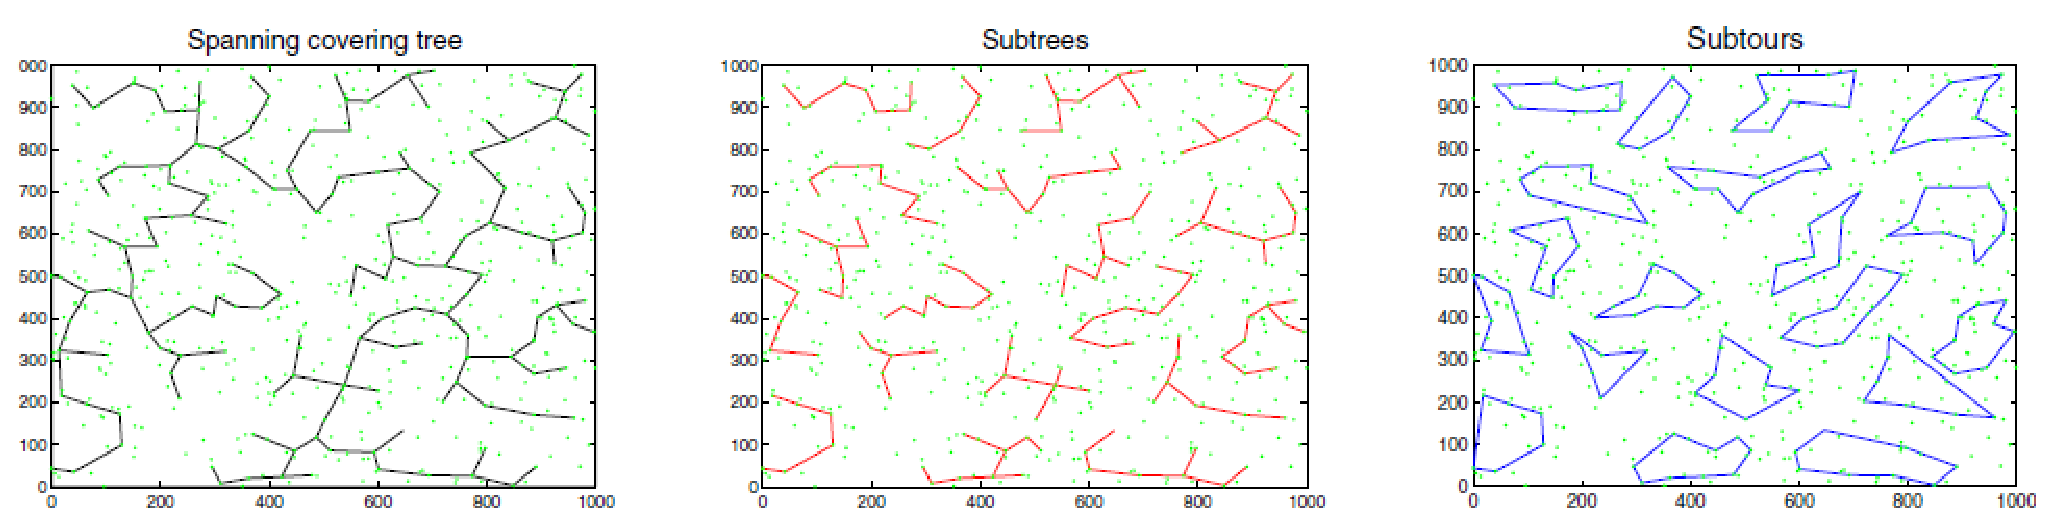
\includegraphics[width=\textwidth]{images/yuanyuan_mst.eps}
	\caption{Τα 3 βήματα του αλγορίθμου.}
	\label{fig:yuanyuan_mst}
\end{figure}
Αρχικά κατασκευάζεται κατανεμημένα ένα ελάχιστο γεννητικό δέντρο με όλους τους κόμβους, το δέντρο αυτό αποσυντίθεται σε μικρότερα ελάχιστα γεννητικά δέντρα, όσες και
οι κινητές Πηγές και αναζητείται σε κάθε τέτοιο δέοντρο το μικρότερο μονοπάτι το οποίο επιεκέπτεται όλους τους κόμβους. Οι κινητές Πηγές στέλνουν τα δεδομένα τους
στην κύρια Πηγή χρησιμοποιώντας της υπόλοιπες κινητές Πηγές. Πειράματα έδιξαν οτι εξοικονομείται σημαντικό ποσό της ενέργειας.


Η εργασία στο \cite{dynamic_deadlines} εξετάζει το πρόβλημα από μια διαφορετική σκοπιά. Οι συγγραφείς αρχικά επισημένουν οτι το πρόβλημα με τις κινητές Πηγές
ουσιαστικά πρόκειται για την δρομολόγηση κινητών με χρονικές προθεσμίες οι οποίες καθορίζονται από τον χώρο μνήμης ενός κόμβου ή πιο αφαιρετικά από το μέγιστο μέγεθος
των δεδομένων κάθε κόμβου θα κρατάει πριν τα παραδώσει στην Πηγή. Υπο αυτή την έννοια το πρόβλημα είναι λίγο διαφορετικό από το TSP πρόβλημα με την έννοια οτι η κάθε
κινητή Πηγή μπορεί να χρειαστεί να επισκεφθεί περισσότερες από μια φορά έναν κόμβο ανάλογα με τον ρυθμό παραγωγής των γεγονότων σε εκείνη την περιοχή. Αφού
αποδείξουν οτι το πρόβλημα είναι NP-complete κατασκευάζουν 3 ευρετικούς αλγορίθμους.
\begin{itemize}
\item \textbf{Νωρίτερη προθεσμία πρώτα:} σε αυτή την περίπτωση ο αλγόριθμος επισκέπτεται πρώτα τον κόμβο του οποίου ο χώρος μνήμης είναι πιο κοντά να ξεχειλείσει. το
πρόβλημα με αυτόν τον ευρετικό αλγόριθμο είναι οτι δεν παίρνει υπόψην του καθόλου το κόστος του κάθε κόμβου για να τον επισκεφθεί, δηλαδή την απόστασή του από την
τωρινή θέση της κινητής Πηγής.
\item \textbf{Νωρίτερη προθεσμία με $k$-κόμβους μπροστά:} σε αυτή την περίπτωση η κινητή Πηγή ταξινομεί τις προθεσμίες όλων των κόμβων και επιλέγει τις $k$
μικρότερες. Στη συνέχεια, επιλέγει την σειρά με την οποία θα επισκεφθεί τους $k$ αυτούς κόμβους έτσι ώστε καμία προθεσμία να μην χαθεί και ταυτόχρονα η συνολική
διαδρομή, δηλαδή ο χρόνος που θα χρειαστεί, να είναι η μικρότερη δυνατή.
\item \textbf{Ελάχιστο ζυγισμένο άθροισμα πρώτα:} σε μία προσπάθεια να εξισορροπήσουν το κόστος απόστασης με την χρονική προθεσμία οι συγγραφείς δημιούργησαν αυτόν
τον υβριδικό ευρετικό αλγόριθμος. Δηλαδή δημιουργούν το διάνυσμα
\begin{align*}
weighted\_sum[i] = & \alpha_{mwsf}\dot (deadline[i]-current\_time[i]) +\\
& (1-\alpha_{mwsf})(cost[current\_position][i])
\end{align*} και επιλέγουν τον κόμβο που έχει την μικρότερη τιμή.
\end{itemize}
Στην συνέχεια συγκρίνουν τους αλγορίθμους αυτούς με έναν αρκετά γνωστό
ευρετικό αλγόριθμο ο οποίος προέρχεται από την δρομολόγηση οχημάτων \cite{vehicle_routing_windows}. Τα βήματα του αλγορίθμου είναι τα εξής:
\begin{enumerate}
\item Ξεκινάει με ένα όχημα και έναν κόμβο ο οποίος είναι ο πρώτος στην διαδρομή του
\item Στην συνέχεια βρίσκει τον καλύτερο κόμβο που μπορεί να εισέλθει στην διαδρομή του
\begin{itemize}
	\item Αυτό συνεχίζεται μέχρι κανένας νέος κόμβος να μην μπορεί να εισέλθει λόγω περιορισμών στις προθεσμίες
\end{itemize}
\item Ο αλγόριθμος τότε προσθέτει ένα νέο όχημα και η διαδικασία συνεχίζεται παρόμοια για το νέο όχημα
\end{enumerate}
 Ο αλγόριθμος αυτός μπορεί να εφαρμοστεί και για την δρομολόγηση των κινητών Πηγών σε ένα ασύρματο δίκτυο αισθητήρων αφού τα 2 προβλήματα είναι παρόμοια.

Μια διαφορετική, ριζοσπαστική προσεγγιση εμφανίστηκε στην εργασία \cite{extending_lifetime_rizo}. Κατ'αρχήν, το μοντέλο της εργασίας υποθέτει έναν κύκλο ακτίνας $R$
μέσα στον οποίο τοποθετούνται ομοιόμορφα κατανεμημένα $N$ κόμβοι. Επίσης όλοι ο κόμβοι οι οποίοι είναι 2-βήματα ή 1-βήμα ( 2-hop ή 1-hop) μακριά από την στατική Πηγή
ανήκουν στο σύνολο $G$. Στην εργασία αυτή οι συγγραφείς εκμεταλεύονται τους κόμβους που ανήκουν στο $G$ "καίγοντάς" τους μέσα από έναν κινητό κόμβο.
\begin{figure}[h]
\begin{subfigure}{0.4\textwidth}
\centering
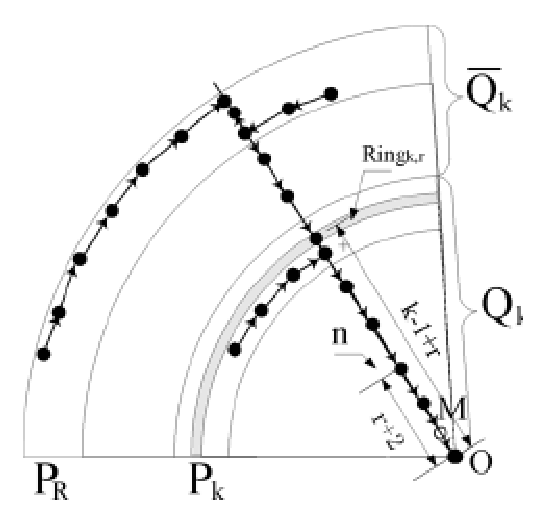
\includegraphics[scale=0.4]{images/extending_lifetime_1.eps}
\caption{}
\label{fig:extending_lifetime_path}
\end{subfigure}
\begin{subfigure}{0.5\textwidth}
\centering
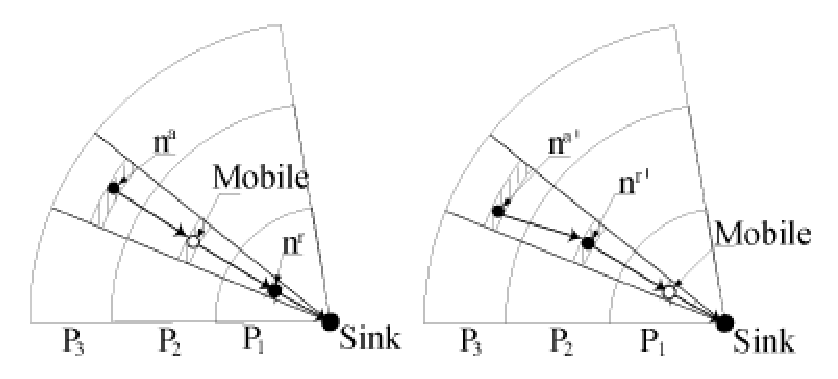
\includegraphics[scale=0.5]{images/extending_lifetime_2.eps}
\caption{}
\label{fig:extending_lifetime_depletion}
\end{subfigure}
\caption{Η διαδρομή που ακολουθούν τα πακέτα (α') και ο τρόπος που εκμεταλεύεται τους 2-hop γείτονες της στατικής Πηγής ο κινητός κόμβος (β'). }
\label{fig:}
\end{figure}
Όπως φαίνεται και στην εικόνα \ref{fig:extending_lifetime_depletion} ο κινητός κόμβος αντικαθιστά κάθε φορά έναν κόμβο από αυτούς που είναι 2-hop ή 1-hop μακριά και
χρησιμοποιεί τον άλλον (ο οποίος βρίσκεται πάνω στην ακτίνα που σχηματίζεται από τον κινητό κόμβο και την στατική Πηγή έστω $r$) μέχρι να του εξαντλήσει τελείως την
ενέργειά του. Κάθε φορά που ο κινητός κόμβος επιλέγει έναν νέο κόμβο $u_{i}\in G$ τότε όλοι οι κόμβοι οι οποίοι ανήκουν στην ακτίνα $r$ λαμβάνουν όλα τα πακέτα από
όλους του κόμβους που ανήκουν στο ίδιο δαχτυλίδι. Δηλαδή οι κόμβοι που ανήκουν σε έναν δακτύλιο στέλνουν τα πακέτα τους πάνω από αυτόν δακτύλιο μέχρι να φτάσουν στον
κόμβο που ανήκει στην ακτίνα $r$ όπως φαίνεται και στην εικόνα \ref{fig:extending_lifetime_path}. Οι συγγραφείς αποδυκνύουν αναλυτικά οτι με αυτό το σχήμα το δίκτυο
μπορεί να έχει χρόνο ζωής  $T>4\frac{E}{R^{2}e}-\frac{16E}{R^{4}e}$ δεδομένου οτι για την ακτίνα του δικτύου $R$ ισχύει $R>16\pi+4$. Χρησιμοποιώντας την ίδια λογική
αποδεικνύεται οτι για $m$ κινητούς κόμβους (οι οποίοι εκμεταλεύονται $2m$ στατικούς κόμβους πάνω στην ακτίνα $r$) ο χρόνος ζωής του δικτύου φράσεται από την σχέση:
\begin{align*}
T>4m\frac{E}{R^{2}e}-frac{32\pi m^{3}E}{R^{4}e} \qquad\text{αν η ακτίνα $R$ είναι αρκετά μεγάλη}
\end{align*}
Τα πειράματα αυτής της εργασίας έδειξαν οτι ο χρόνος ζωής αυξάνεται σημαντικά και επαληθεύονται τα προηγούμενα θεωρητικά αποτελέσματα. Όπως έγινε εμφανές η εργασία
αυτή ακολουθεί μια διαφορετική λογική από τις υπόλοιπες σχετικές εργασίες το οποίο την κάνει ξεχωριστή.

Μια επίσης διαφορετική εργασία στο \cite{auction_energy_balance}. Στην εργασία αυτή θεωρείται ένα υβριδικό δίκτυο αισθητήρων το οποίο αποτελείται από κινητούς
κόμβους και στατικούς κόμβους. Στο μοντέλο θεωρείται οτι οι κινητοί κόμβοι έχουν πολύ περισσότερη ενέργεια από τους στατικούς, ο χρόνος χωρίζεται σε γύρους και η
εργασία επικεντρώνεται στην κατάλληλη διαχείρηση των κινητών κόμβων σε έναν γύρο. Να σημειωθεί οτι αποτελεί από τις λίγες εργασίες που παίρνει υπόψην στο μοντέλο της
και στοχεύει στην μείωση της κατανάλωσης την ενέργεια που σπαταλάται για την κίνηση ενός κινητού κόμβου. Οι συγγραφείς προτείνουν αρχικά έναν καθολικό (centralized)
αλγόριθμο και στην συνέχεια έναν κατανεμημένο αλγόριθμο. O κατανεμημένος αλγόριθμος χρησιμοποιεί μια διαφορετική προσέγγισει για να λύσει το πρόβλημα της
δρομολόγησης των κινητών κόμβων. Αρχικά η περιοχή του δικτύου χωρίζεται σε ένα πλέγμα (grid) και κάθε κελί εκλέγει έναν στατικό κόμβο ως αρχηγό. Ο χρόνος χωρίζεται
περεταίρω σε 3 διαφορετικές φάσεις ενός γύρου:
\begin{itemize}
\item \textbf{Φάση διάδοσης:} Αρχικά ο αρχηγός κάθε κελιού μέσα στο πλέγμα συλλέγει τις τοποθεσίες των γεγονότων από τους στατικούς αισθητήρες. Επίσης συλέγει τις
αναφορές (τοποθεσία, ενέργια) των κινητών κόμβων. Στην συνέχεια η ύπαρξη των κινητών κμόβων διαφημίζεται από τα κελιά που τους περιέχουν.
\item \textbf{Φάση διαγωνισμού:} Κάθε κελί του πλέγματος που περιέχει ένα γεγονός (και επομένως πρέπει να έρθει ένας κινητός κόμβος για να το συλλέξει) διαγωνίζεται
με όλα τα άλλα αντίστοιχα κελιά για τους κινητούς κόμβους χρησιμοποιώντας προσκλήσεις. Ο κάθε κινητός κόμβος αποδέχεται ή απορρήπτει μια πρόσκληση ανάλογα με τα
δεδομένα της πρόσκλησης όπως π.χ η απόσταση του γεγονότος από τη θέση του κινητού κόμβου.
\item \textbf{Φάση δρομολόγησης:} Ο κάθε κινητός κόμβος αφού έχει επιλέξει μια σειρά από κελιά τότε εκτελεί την διαδρομή του χρησιμοποιώντας προσεγγιστικό αλγόριθμο
του προβλήματος TSP.
\end{itemize}
Αποδεικνύεται οτι η πολυπλοκότητα του αλγορίθμου είναι $O(m\cdot\hat{M} + n\cdot\hat{N} + m^{2}h)$ όπου $m,n$ οι κινητοί και στατικοί κόμβοι αντίστοιχα, $\hat{M},
\hat{N}$ οι διαστάσεις του πλέγματος και $h$ η διάμετρος του δικτύου. Οι προσομοιώσεις δείξαν οτι υπάρχει σημαντική αύξηση του χρόνου ζωής του δικτύου.



\section{Εναλλακτικές Τεχνικές} % node density(normal distribution)
Εκτός από τους αλγόριθμους δρομολόγησης υπάρχουν και άλλες τεχνικές που έχουν μελετηθεί με σκοπό την επέκταση του χρόνου ζωής ενός ασύρματου δικτύου αισθητήρων.
Έχουν μελετηθεί τεχνικές που έχουν να κάνουν με αξοιοποίηση εναλλακτικών πηγών ενέργειας όπως είναι η ηλιακή ενέργεια, τεχνικές που θεωρούν πιο ισχυρά μοντέλα όπως
η πρόσθεση επιπλέον κόμβων σε ένα δίκτυο εκεί που χρειάζεται αλλά και τεχνικές... Τέλος παρουσιάζεται μια νές πρωτοπόρα ριζοσπαστική τεχνική, αυτή της ασύρματης
φόρτισης, η οποία αναλύεται εκτενέστερα στο κεφάλαιο \ref{ch:wrsns}.

\subsection{Τεχνικές εναλλακτικών πηγών ενέργειας}
Οι τεχνικές αυτές ασχολούνται με την αξιοποίηση εναλλακτικών πηγών ενέργειας (energy harvesting) προκειμένου να φορτίσουν τους στατικούς κόμβους που επιβλέπουν το
περιβάλλον. τα τελευταία χρόνια αυτές οι τεχνικές έχουν γνωρίσει μεγάλη ανάπτυξη και έχουν ενσωματωθεί επιτυχημένα σε συστήματα ΑΔΑ. Υπάρχει ποικιλία διαφορετικών
ενεργειών που μπορούν να χρησιμοποιηθούν για την αύξηση ζωής του δικτύου όπως μηχανική, θερμική και ηλιακή ενέργεια η οποία μπορεί να μετατραπεί σε ηλεκτρική και να
ενεργοποιήσει τους κόμβους ή απλώς να επαναφορτήσει τις μπαταρίες τους. Η πιο πολυχρησιμοποιούμενη είναι η ηλιακή ενέργεια. Για την ηλιακή ενέργεια ο ρυθμός
επαναφόρτισης ορίζεται από τον παρακάτω τύπο:
\begin{align*}
\pi_{r} = Rad_{s} \times \eta_{\rho} \times \rho_{e} \times A
\end{align*}
όπου to $Rad_{s}$ αντιστοιχεί στην ηλιακή ακτινοβολία, το $\eta_{\rho}$ αντιστοιχεί στην αποδοτικότητα του ηλιακού συλλέκτη να μετατρέψει την ηλιακή ενέργεια σε
ηλεκτρική ενέργεια, το $\rho_{e}$ αντιστοιχεί στην απόδοση του ηλεκτρικού κυκλώματος και το $A$ αντιστοιχεί στο μέγεθος του ηλιακού συλλέκτη.

Ωστόσο καθώς όλες αυτές οι εναλλακτικές ενέργειες προέρχονται από το εξωτερικό περιβάλλον οι χωροχρονικοί χαρακτήρες τους έχουν μεγάλες διακυμάνσεις όσον αφορά την
απόδοση τους η οποία συνήθως είναι χαμηλή και ευέσθητη στην δυναμική του περιβάλλοντος. Για παράδειγμα σε ένα σύστημα βασισμένο στην ηλιακή ενέργεια, η ισχύς εξόδου
του η οποία θα τροφοδοτήσει έναν αισθητήρα καθορίζεται από τις ηλιακές ακτίνες που προσάπτονται εκείνη την στιγμή στους ηλιακούς συλλέκτες και μεταβάλλεται σημαντικά
ανάλογα με την ώρα και τον καιρό. Στατιστικές έχουν δείξει οτι υπάρχει διαφορά μέχρι και 3 τάξεις μεγέθους στην διαθέσιμη ενέργεια ανάμεσα σε μια σκιώδης,
συννεφιασμένης και ηλιόλουστης μέρας \cite{harvesting_comparison}. Καθώς δεν υπάρχει γενικά τρόπος να γνωρίζει εξ'αρχής κανείς την κατάσταση που θα υπάρχει στο δίκτυο
αισθητήρων υπάρχει μεγάλη δυσκολία στο σχεδιασμό πρωτοκόλλων που εκμεταλεύονται τέτοιες μορφές ενέργειας και να κρατάνε τους κόμβους πάντα ενεργούς. Αυτό όμως είναι
πολύ δύσκολο ειδικά σε εφαρμογές στις οποίες το κύριο έργο είναι να συλλέγουν περιοδικά δεδομένα και πληροφορίες από όλους τους κόμβους. Στην περίπτωση που κάποιοι
αισθητήρες καταναλώσουν όλη την ενέργειά τους και δεν επαναφορτιστούν γρήγορα, το δίκτυο σταδιακά θα καταρεύσει. Υπάρχουν όμως πρωτόκολλα που ρυθμίζουν τις
λειτουργίες του κάθε κόμβου ανάλογα με την κατάσταση που επικρατεί στο εξωτερικό του περιβάλλον και παρουσιάζονται στην συνέχεια.

Μία από τις πρώτες εργασίες παρουσιάζεται στο \cite{heliomote}. Στην εργασία αυτή παρουσιάζεται ένα σύστημα του οποίου οι κόμβοι έχουν ηλιακούς συλλέκτες
και μπορούν να φορτίζονται από την ηλιακή ενέργεια όπως φαίνεται στην εικόνα \ref{fig:heliomote_example}.
\begin{figure}[h]
	\centering
	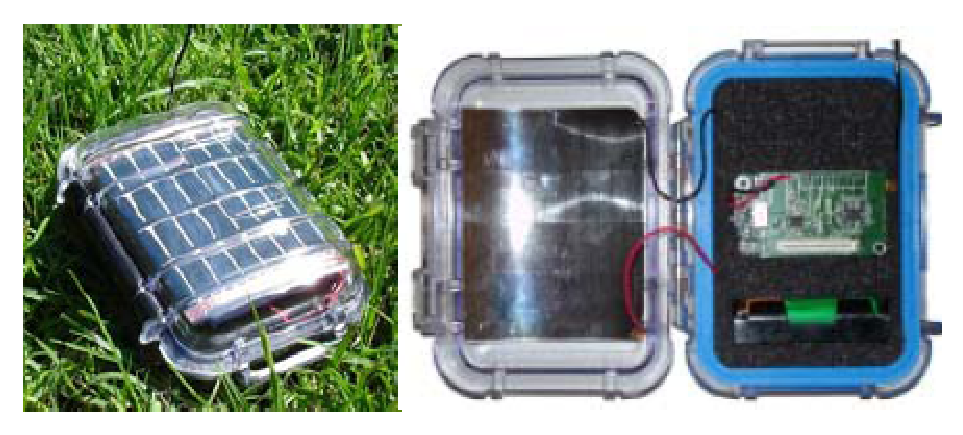
\includegraphics[width=0.8\textwidth]{images/heliomote_example.eps}
	\caption{Ένας κόμβος του συστήματος \textit{Heliomote}.}
	\label{fig:heliomote_example}
\end{figure}

Με αυτόν τον τρόπο το σύστημα μπορεί να επιμηκύνει το χρόνο ζωής του συλλέγοντας ενέργεια από τον ήλιο. Επιπλεόν στην εργασία προτείνεται ένας εναλλακτικός τρόπος
δρομολόγησης των πακέτων. Συγκεκριμένα, τα πακέτα δρομολογούνται μέσα από μονοπάτια τα οποία έχουν το μεγαλύτερη συλλογή ηλιακής ενέργειας. Επίσης κόμβοι οι οποίοι
έχουν μικρή συλλογή ηλιακής ενέργειας (π.χ. είναι κάτω από ένα δέντρο) τότε μειώνουν τον φόρτο εργασίας τους εσκεμένα. Υπάρχει επομένως εξισορρόπηση της ενέργειας
του δικτύου.

Στην εργασία \cite{harvesting_6} μελετάται η περίπτωση ενός ασύρματου δικτύου αισθητήρων στο οποίο υπάρχει πλεονασμός κόμβων οι οποίοι μπορούν να
επαναφορτιστούν. Η εργασία αναλύει το πρόβλημα του πως οι κόμβοι θα έπρεπε να ενεργοποιούνται δυναμικά έτσι ώστε να μεγιστοποιηθεί η κάλυψη του δικτύου. Αφού δειχθεί
η βέλτιστη λύση, στην συνέχεια προτείνεται μια κατανεμημένη πολιτική ενεργοποίησης η οποία επιτυγχάνει το $\frac{3}{4}$ της βέλτιστης λύσης ενώ παρέχονται
προσομοιώσεις που επιβεβαιώνουν τα θεωρητικά αποτελέσματα.

Στην εργασία \cite{harvesting_7} αναλύεται η απόδοση πολυ-βηματικών (multi-hop) μεταδόσεων στην περίπτωση που υπάρχει δυνατότητα επαναφόρτισης ορισμένων κόμβων. Στην
συνέχεια σχεδιάζεται ένας αλγόριθμος ο οποίος λαμβάνει υπόψην του την αναπλήρωση ενέργειας των κόμβων και προωθεί τα πακέτα προς αυτούς τους κόμβους ο οποίος είναι
ασυμπτωτικά βέλτιστος σε αντιστοιχία με το μέγεθος του δικτύου. Ο αλγόριθμος δεν θεωρεί κάποια στατιστική πληροφορία όσον αφορά την άφιξη των πακέτων και επομένως
μπορεί να ενσωματωθεί σε ήδη υπάρχοντα σχήματα δρομολόγησης (προληπτικά ή κατ'απαίτηση). Τα αποτελέσματα των προσομειώσεων επιβεβαιώσαν οτι ο αλγόριθμος πετυχαίνει
να μεγιστοποιήσει την απόδοση σε ενεργειακά (energy-aware) δίκτυα.

Στις εργασίες \cite{harvesting_8} \cite{harvesting_9} αναλύεται ξανά η βέλτιστη δειγματοληψία των κόμβων κάτω από τους περιορισμούς των εναλλακτικών ενεργειών όπως
είναι η φωτεινότητα στην ηλιακή ενέργεια. Σε κάθε περίπτωση προτείνεται ένας κατανεμημένος αλγόριθμος ο οποίος ρυθμίζει κατάλληλα τον ρυθμό δειγματοληψίας του κάθε
κόμβου και λύνει το πρόβλημα αποδοτικά. Τέλος εκτελούνται προσομοιώσεις που αποδεικνύουν την απόδοση του εκάστοτε αλγορίθμου.



\subsection{Τεχνικές αυξησης των κόμβων του δικτύου}
Στην τεχνική αυτή υπάγονται εργασίες οι οποίες αναλύουν την βέλτιστη κατανομή των κόμβων σε ένα ασύρματο δίκτυο αισθητήρων και εργασίες που προτείνουν αποδοτικούς
τρόπους για την αντικατάσταση κόμβων του δικτύου οι οποίοι έχουν χάσει πλήρως την ενέργειά τους. Στην πρώτη περίπτωση εκτελείται ένας προληπτικός αλγόριθμος (offline
algorithm) ο οποίος βρίσκει την βέλτιστη την βέλτιστη ανάπτυξη των αισθητήρων κάτω από συγκεκριμένες συνθήκες. Στη δεύτερη περίπτωση εκτελούνται αλγόριθμοι άμεσης
απόκρισης (online algorithms) οι οποίοι αφού αναλύσουν την κατάσταση του δικτύου, βρίσκουν το βέλτιστο υποσύνολο του δικτύου το οποίο θα πρέπει να αντικατασταθεί ή
να προστεθούν επιπλέον κόμβοι.

Στην εργασία \cite{gaussian_sensors} οι συγγραφείς αναλύουν την περίπτωση όπου οι κόμβοι δεν τοποθετούνται ομοιόμορφα κατανεμημένα αλλά με βάση την Gaussian κατανομή
σε δισδιάστατιο χώρο. Στην συνέχεια εντοπίζουν κάτω από συγκεκριμένες υποθέσεις και ιδιότητες της Gaussian κατανομής μπορεί να επιτευχθεί η επιθυμητή καλυψη και
διάρκεια ζωής του δικτύου. Αφού αναλύσουν τις στρατηγικές ανάπτυξης των κόμβων προτείνουν 2 αλγόριθμους ανάπτυξης των κόμβων οι οποίοι αυξάνουν σημαντικά τον χρόνο
ζωής του δικτύου.

Η εργασία στο \cite{sens_deployment3} εισάγει για πρώτη φορά στο μοντέλο των ΑΔΑ την έννοια της πρόσθεσης ή αντικατάστασης κόμβων του δικτύου ενώ ενσωματώνει στο
μοντέλο την έννοια της ετερογένειας, της ύπαρξης δηλαδή διαφορετικών κόμβων ως προς τις δυνατότητές τους. Με τις προαναφερθείσες παραδοχές αυξάνεται σημαντικά η
δυναμικότητα του δικτύου που μελετάται και οι συγγραφείς διαπιστώνουν οτι ο μόνος τρόπος για την αποδοτική διαχείρηση της ενέργειας είναι μέσα από αλγόριθμους
μάθησης. Συγκεκριμένα, οι συγγραφείς αναπτύσουν έναν κατανεμημένο αλγόριθμο ελαχιστοποίησης της ενέργειας ο οποίος χρησιμοποιεί τοπικές πληροφορίες όπως για
παράδειγμα πυκνότητα και ενέργεια του δικτύου σε μια τοπική περιοχή και ρυθμίζει κατάλληλα την πολιτική ύπνου (sleeping policy) των κόμβων. Οι προσομειώσεις δείξαν
οτι με αυτόν τον τρόπο διπλασιάζετα σχεδόν ο λόγος επιτυχίας σε σύγκριση με το Directed Diffusion ενώ μαζί με την προσθήκη ετερογενών κόμβων σε κατάλληλα σημεία του
δικτύου ο λόγος επιτυχίας αυξάνεται ακόμα περισσότερο με παρόμοια ενεργειακή συμπεριφορά.

Η εργασίες στα \cite{sens_deployment1} \cite{sens_deployment2} μελετάνε την περίπτωση ενός δικτύου το οποίο λειτουργεί για πολύ μεγάλο χρονικό διάστημα. Για να
λύσουν το πρόβλημα που δημιουργείται από τους περιορισμένους πόρους ενέργειας που έχει ο κάθε κόμβος προτείνουν μια στρατηγική αντικατάστασης και ανάκτησης των παλιών
κόμβων με καινούργιους. Για την υλοποίηση της ιδέας χρησιμοποιείται ένα μηχανικά κινούμενο ρομπότ το οποίο έχει την ικανότητα να αντικαθιστά τους κόμβους του
δικτύου. Το ρομπότ αυτό περιοδικά διασχίζει την περιοχή του δικτύου και εγκαθιστά καινούργιους κόμβους ενώ επιστρέφει τους παλιούς κόμβους στην βάση για επαναφόρτηση.


\subsection{Τεχνικές επαναφόρτισης κόμβων} \label{sc:recharg_tecnhiques}
Η πρόσφατη πρόοδος στις περιοχές των υλικών που χρησιμοποιούνται για τις μπαταρές αλλά και στην περιοχή της ασύρματης μετάδοσης ενέργειας προσφέρουν νέες δυνατότητες
διαχείρησης της διαθέσιμης ενέργειας. Στην πρώτη περιοχή ανακαλύφθηκε ένα νέο υλικό για μπαταρίες το οποίο επιτρέπει πολύ γρήγορες φορτίσεις και αργές ξεφορτίσεις
\cite{fast_recharging}. Η ανακάλυψη αυτή συνδυάζει τα πλεονεκτήματα των κλασσικών $Li-ion$ μπαταριών και των υπερ-πυκνωτών χρησιμοποιώντας την τεχνολογία
$LiFePO_{4}$ επιτρέποντας φορτίσεις μέχρι και 400C\footnote{C ορίζεται ως η ονομαστική χωρητικότητα της μπαταρίας. Για παράδειγμα για μία
μπαταρία χωρητικότητας 1000mAh C=1000mA.}. Στη δεύτερη περιοχή η τεχνολογία γύρω από την ασύρματη μετάδοση ενέργειας έχει εξελιχθεί τόσο πολύ που πλέον τα ποσοστά
επιτυχίας έχουν ανέβει σημαντικά. Οι εργασίες στα \cite{wireless_recharg1}, \cite{wireless_recharg2}, \cite{wireless_recharg3} δείχνουν οτι μπορεί να υπάρξει μέχρι
και 60\% απόδοση στην μεταφορά ενέργειας. Ταυτόχρονα η Intel\textsuperscript{\textregistered} δείχνει μέχρι και 75\% απόδοση \cite{intel_recharg} ενώ η εταιρεία
Witricity\textsuperscript{\textregistered} ισχυρίζεται οτι μπορεί να επιτύχει μεταφορά ενέργειας με ποσοστό επιτυχίας μέχρι και 90\% \cite{witricity_90}. Η
συγκεκριμένη τεχνολογία έχει οδηγήσει σε έναν καινούργιο κλάδο των ασύρματων δικτύων ασιθητήρων: τα ασύρματα επαναφορτιζόμενα δίκτυα αισθηρήτων (ΑΕΔΑ). Θα αναλυθεί
εκτενέστερα στο επόμενο κεφάλαιο αφού αποτελεί τον κηνητήριο μοχλό για αυτή την διπλωματική εργασία.

























%3rd chapter


\chapter{Ασύρματα Επαναφορτιζόμενα Δίκτυα Αισθητήρων (ΑΕΔΑ)}
\section{Τεχνολογία}
\label{ch:wrsns}
%4th chapter


\chapter{Ορισμός του Προβλήματος και Ιδιότητές του}
\section{Ορισμός}
\subsection{Γενικευμένος ορισμός}
\subsection{Παραλλαγές του Προβλήματος}

\section{Ιδιότητες του Προβλήματος}
\subsection{Απόδειξη της Δυσκολίας Επίλυσης του Προβλήματος}
\subsection{Ένα άνω φράγμα}

%5rd chapter


\chapter{Στρατηγικές και Αλγόριθμοι}
\label{ch:strategies-and-algorithms}
%6th chapter


\chapter{Πειραματική Αξιολόγηση}
\label{ch:results}
%7th chapter


\chapter{Επίλογος και Ανοιχτά Προβλήματα}\label{ch:conclusion}
\section{Ανασκόπηση και Συμπεράσματα}

\section{Μελλοντικές Αναζητήσεις}

%bibliography to do later
%\bibliographystyle{plain}
% \bibliography{thesis}

\end{document}